% TODO: standardized equation notation. Is it eqn, Eqn, Eq? (all three are used).



\chapter{Allele and genotype frequencies}
 In this chapter we will
work through how the basics of Mendelian genetics play out at the population
level in sexually reproducing organisms.The genome of an individual is formed from two gametes that fused to form a zygote. In turn, the genomes of each gamete originate from a parental genome through meiosis, in particular the segregation
and recombination of the parental genome's two gametes. 
Loci and alleles are the basic currency of population genetics--and indeed of
genetics. Each individual's genetic makeup is defined in their genome. \marginnote[-1cm]{A
\emph{locus} (plural: \emph{loci}) is a specific spot in the genome. A locus
may be an entire gene, or a single nucleotide base pair such as A-T. At each
locus, there may be multiple genetic variants segregating in the
population---these different genetic variants are known as \emph{alleles}.} If
all individuals in the population carry the same allele, we say that the locus
is \emph{monomorphic}; at this locus there is no genetic variability in the
population. If there are multiple alleles in the population at a locus, we say
that this locus is \emph{polymorphic} (this is sometimes referred to
as a segregating site).

Table \ref{Table:ADH} show a small stretch orthologous sequence for
the ADH from samples from {\it Drosophila melanogaster},  {\it D. simulans},
and {\it D. yakuba}.  {\it D. melanogaster} and {\it D. simulans} are
sister species, with  {\it D. yakuba} being close outgroup to the two.  Each column represents a single haplotype from an
individual (the individuals are diploid but were inbred so they're
homozygous for their haplotype). Only sites that differ among
individuals of the three species are shown. Site $834$ is an example
of a polymophism, some  {\it D. simulans} individuals carry a $C$
allele while others have a $T$. {\emph Fixed differences}  are sites that differ between the species but are monomorphic within
  the species. For example site $781$ is a fixed difference between
  {\it D. melanogaster} and the other two species. 


\begin{question}
{\bf A)} How many segregating sites does the sample from {\it
  D. simulans} have in the ADH gene?\\ 
{\bf B)} How many fixed differences are there between {\emph D. melanogaster} and {\emph D. yakuba}?
%What is the per base divergence are there between {\emph D. melanogaster} and {\emph D. yakuba}?
\end{question}

We can also annotate the alleles and loci in various ways. For example position
$781$ is a non-synonymous fixed difference. We call the less common
allele at a polymorphism the  {\emph minor allele} and the common
allele the {\emph major allele}, e.g. at site $1068$ the $T$ allele is the
minor allele in {\it D. melanogaster}. We call the more evolutionary
recent of the two alleles the {\emph derived allele} and the older of
the two the {\emph ancestral allele}. The $T$ allele at our site is
the derived allele as the $C$ is found in both the other species,
suggesting that the $T$ allele arose via a $C \leftarrow T$ mutation.

% For example, at a particular nucleotide site in the genome, a population may segregate for A-T and G-C base pairs (note that due to the complementary nature of DNA, it will suffice to say the site segregates for A and G variants).

\begin{table*}
  \tiny
\setlength{\tabcolsep}{.45\tabcolsep}   % https://tex.stackexchange.com/questions/307770/centered-tabular-column-with-narrow-columns
 %\csvreader[tabular=c]{Journal_figs/alleles_genotypes/ADH_MK/ADH.csv}
\csvautobooktabular{Journal_figs/alleles_genotypes/ADH_MK/ADH.csv}  % can control this more https://mirror.hmc.edu/ctan/macros/latex/contrib/csvsimple/csvsimple.pdf
  \caption{Variable sites in exons 2 and 3 of the ADH gene in {\it Drosophila} \citet{mcdonald:91}.  
The first column (pos.) gives the position in the gene, exon 2 begins at
position 778 and exon 3 begins at position 942.
The second column gives the consensus nucleotide (con.), i.e. the most
common base at that position; individuals with nucleotides that match
the consensus are marked with a dash.  The first columns of sequence
(a-l) are from {\it D. melanogaster};
    the next columns (a-f) give sequences from {\it D. simulans}, the final 
 set of coumns (a-l ) from {\it D. yakuba}. The last column shows
 whether the difference is a non-synonymous (N) or synonymous change. }  % I've dropped the
                                % heterozygote sites from D. yakuba.
  \label{Table:ADH}
\end{table*}



\section{Allele frequencies}
Allele frequencies are a central unit of population genetics
analysis, but from diploid individuals we only get to observe genotype
counts. Our first task then is to calculate allele frequencies from
genotype counts. Consider a diploid autosomal locus segregating at two alleles ($A_1$ and
$A_2$). We'll use these arbitrary labels for our alleles, merely to keep this
general. Let $N_{11}$ and $N_{12}$ be the number of $A_1A_1$ homozygotes and
$A_1A_2$ heterozygotes, respectively. Moreover, let $N$ be the total number of
diploid individuals in the population. We can then define the relative
frequencies of $A_1A_1$ and $A_1A_2$ genotypes as $f_{11} = N_{11}/N$ and
$f_{12} = N_{12}/N$, respectively. The frequency of allele $A_1$ in the
population is then given by

\begin{equation}
  p = \frac{2 N_{11} + N_{12}}{2N} = f_{11} + \frac{1}{2} f_{12}. 
\end{equation}
Note that this follows directly from how we count alleles given individuals'
genotypes, and holds independently of Hardy--Weinberg proportions and
equilibrium (discussed below). The frequency of the alternate allele ($A_2$) is
then just $q=1-p$.

\subsection{Measures of genetic variability}
\paragraph{Nucleotide diversity ($\pi$)}
One common measure of genetic diversity is the average number of single
nucleotide differences between haplotypes chosen at random from a
sample. This is called Nucleotide diversity and often denoted by
$\pi$. 

This measure will depend on the length of sequence it is calculated
for. Therefore, $\pi$ is usually normalized by the length of sequence,
to be a per site (or per base) measure. 

\paragraph{Number of segregating sites.} Another measure of genetic variability is the total number of sites
that are polymorphic (segregating) in our sample. One issue is that
the number of segregating sites will grow as we sequence more
individuals (unlike $\pi$), we'll talked about how to standardize the
number of segregating sites for the number of individuals sequenced
later in the notes (see eqn \eqref{watterson_theta}).

\paragraph{The frequency spectrum.}
We also often want to compile information about the frequency of
alleles across sites.  We call alleles that are found once in a sample
{\emph singletons}, alleles that are found twice in a sample {\emph
  doubletons}, and so on. We count up the number of loci where an
allele is found $i$ times out of $n$, e.g. how many singletons are
there in the sample, and this is called the {\emph frequency
  spectrum}. We'll want to do this in some consistent manner, so we
often calculate the minor allele frequency spectrum, or the frequency
spectrum of derived alleles. \graham{Plot a simple freq. spectrum for
  ADH? And add $\pi$ calc. }

\paragraph{Levels of genetic variability across species.}
Two observations have puzzled population geneticists since the
inception of molecular population genetics. The first is the relatively high
level of genetic variation observed in most obligately sexual species.  
This first observation, in part, drove the devleopment of the Neutral
theory of molecular evolution, the idea that much of this molecular
polymorphism may simply reflect a balance between genetic drift and
mutation. 
The second observation is the relatively narrow range of
polymorphism across species with vastly different census sizes. This
observation represented puzzle as Neutral theory predicts that
levels of genetic diversity should scale population size. Much effort
in theoretical and empirical population genetics has been devoted to
trying to reconcile models with these various observations. We'll
return to discuss these ideas throughout our course.



\begin{marginfigure}
\begin{center}
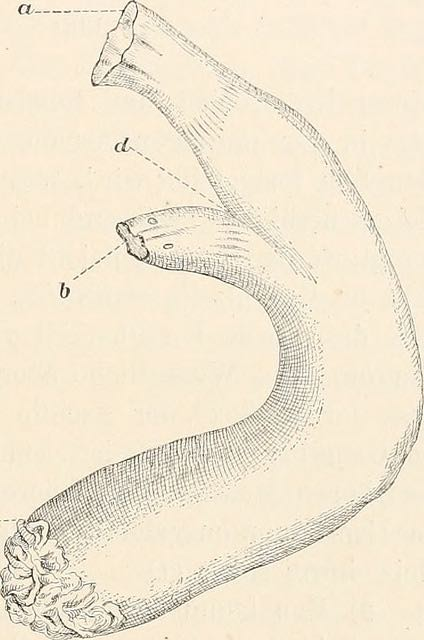
\includegraphics[width= 0.8 \textwidth]{illustration_images/alleles_genotypes/Ciona_intestinalis/21016139168_2a8a57ded3_z.jpg}
\end{center}
\caption{Sea Squirt ({\it Ciona intestinalis}). Einleitung in die vergleichende gehirnphysiologie und
  Vergleichende psychologie. Loeb, J. 1899. } \label{fig:Lynx}
\end{marginfigure}

\begin{marginfigure}
\begin{center}
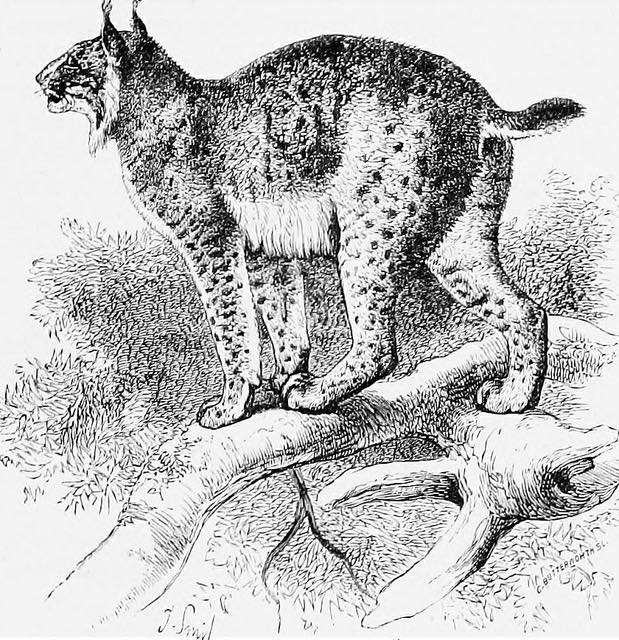
\includegraphics[width= 0.8 \textwidth]{illustration_images/alleles_genotypes/Lynx/20731949565_8a065700af_z.jpg}
\end{center}
\caption{Eurasian Lynx ({\it Lynx lynx}). An introduction to the study
  of mammals living and extinct. Flower, W.H. and Lydekker, R. 1891.} \label{fig:Lynx}
\end{marginfigure}

These observations were first raised from surveys of allozyme data within
natural populations but we can revisit them with modern data. For
example, \citet{leffler:12} compiled data on levels of within-population,
autosomal nucleotide diversity ($\pi$) for 167 species across 14 phyla from
non-coding or synonymous sites (Figure \ref{fig:Leffer}). The species with the lowest levels of
$\pi$ in their survey was Lynx, with $\pi = 0.01\%$, i.e. only
$1/10000$ bases differed between two sequences. While the some of the highest levels of
diversity were found in {\it Ciona savignyi}, Sea Squirts, where a remarkable
$1/12$ bases differ between pairs of sequences. This $800$-fold range of
diversity seems impressive, but census population sizes have a much
larger range.   
\begin{figure*}
\begin{center}
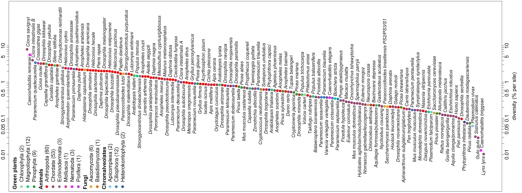
\includegraphics[width= \textwidth]{Journal_figs/alleles_genotypes/Leffer_riddle/Leffer_riddle_diversity.pdf}
\end{center}
\caption{Levels of autosomal nucleotide diversity for 167
species across 14 phyla. Figure 1 from \citet{leffler:12}. Points are
ranked by their $\pi$, and coloured by their phylum. Note the log-scale.} \label{fig:Leffer}
\end{figure*}



\subsection{Hardy--Weinberg proportions}
Imagine a population mating at random with respect to genotypes, i.e. no
inbreeding, no assortative mating, no population structure, no sex differences
in allele frequencies. The frequency of allele $A_1$ in the population at the
time of reproduction is $p$. An $A_1A_1$ genotype is made by reaching out into
our population and independently drawing two $A_1$ allele gametes to form a
zygote. Therefore, the probability that an individual is an $A_1A_1$ homozygote
is $p^2$. This probability is also the expected frequency of the $A_1A_1$
homozygote in the population. The expected frequency of the three possible
genotypes is

%\begin{table}[htp!]
\begin{center}
\begin{tabular}{ccc}
\hline
$f_{11}$ & $f_{12}$ & $f_{22}$ \\
\hline
$p^2$ & $2pq$ & $q^2$ \\
\end{tabular}
\end{center}
%\caption{\textbf{Hardy Weinberg}} \label{table:HWE}
%\end{table}
Note that we only need to assume random mating with
respect to our alleles in order for these expected frequencies to hold,
as long at $p$ is the frequency of the $A_1$ allele in the population at
the time when gametes fuse. 

\begin{question}
On the coastal islands of British Columbia there is a subspecies of
black bear ({\it Ursus americanus kermodei}, Kermode's bear). Many members of this
black bear subspecies are white; they're sometimes called spirit bears. These
bears aren't hybrids with polar bears, nor are they albinos, they are
homozygotes for a recessive change at the MC1R gene. Individuals who
are $GG$ at this SNP are white while $AA$ and $AG$ individuals are black.   

\begin{marginfigure}
\begin{center}
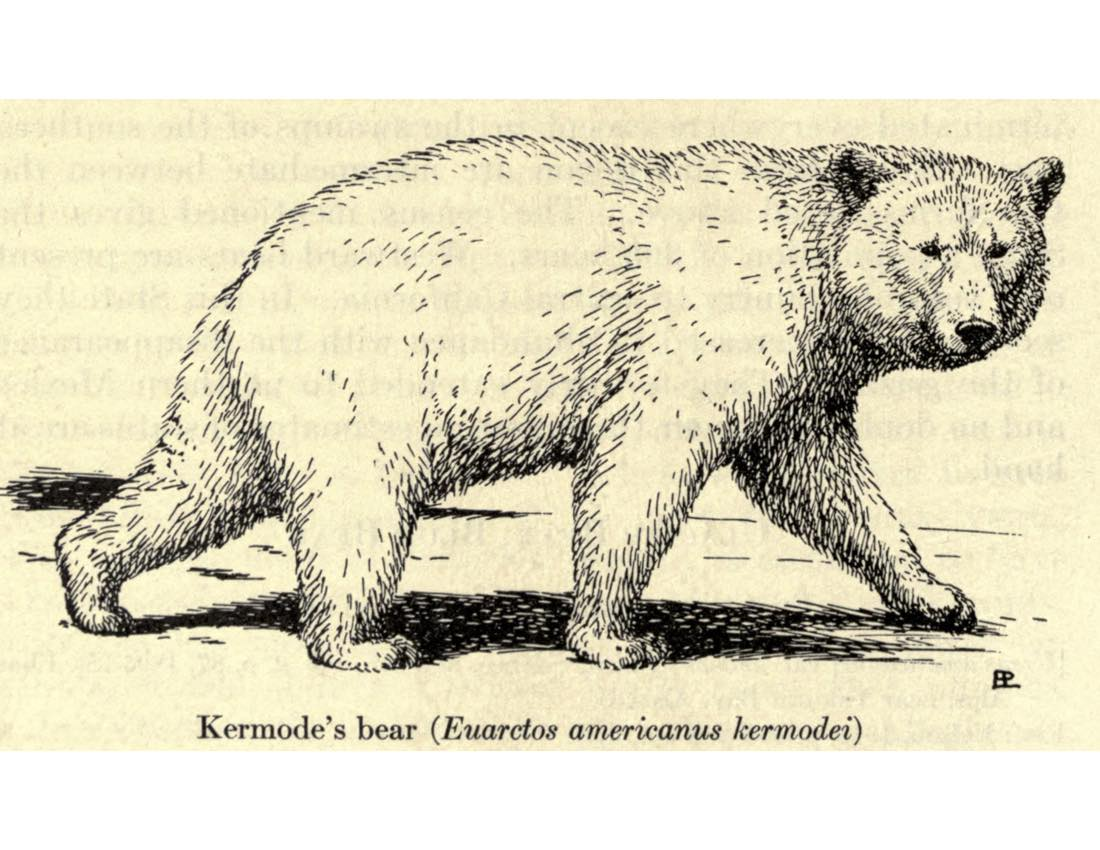
\includegraphics[width= \textwidth]{illustration_images/alleles_genotypes/Kermode_bear/Kermode_bear.pdf}
\end{center}
\caption{Kermode's bear. Extinct and vanishing mammals of the western
  hemisphere. A, Glover 1942.} \label{fig:Kermodes_bear}
\end{marginfigure}

Below are the genotype frequencies for the MC1R polymorphism on from a
sample from British Columbia island populations from \citeauthor{RITLAND:01}. 
\begin{center}
\begin{tabular}{ccc}
\hline
$AA$ & $AG$ & $GG$ \\
\hline
42 & 24 & 21\\
\end{tabular}
\end{center}
Calculate the expected frequencies of the allele under HWE.  
\end{question}


See Figure \ref{fig:HWE_CEU_YRI} for a nice
empirical demonstration of Hardy-Weinberg proportions. 

\begin{figure}[!h]
\begin{center}
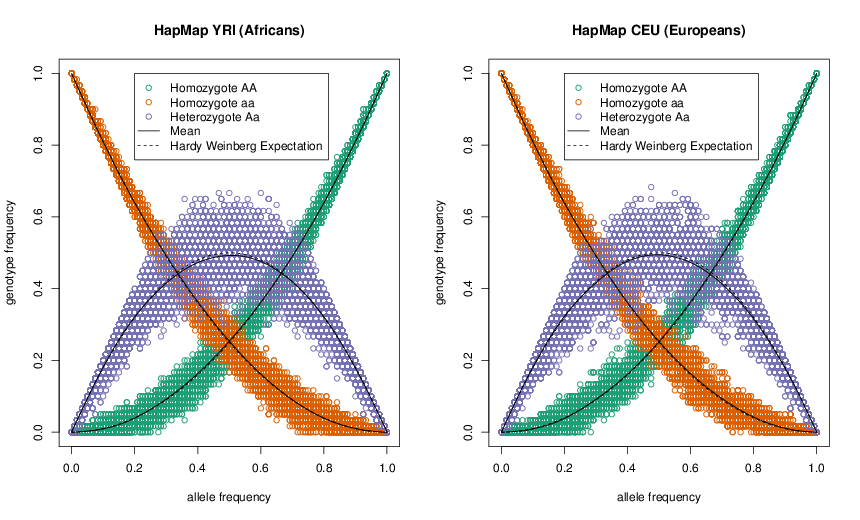
\includegraphics[width= \textwidth]{figures/CEU_YRI_separately_HWE.png} 
\end{center}
\caption{Demonstrating Hardy--Weinberg proportions using 10,000 SNPs
  from the HapMap CEU European and YRI African populations. Within
  each of these populations I plot the allele frequency against the
  frequency of the 3 genotypes. Each SNP is represented by 3 different
  coloured points. The solid lines show the mean genotype frequency. The dashed line shows the
  predicted genotype frequency from Hardy--Weinberg equilibrium.See \href{blog post}{http://gcbias.org/2011/10/13/population-genetics-course-resources-hardy-weinberg-eq/} here on this plot. } \label{fig:HWE_CEU_YRI}
\end{figure}


\marginnote{
\begin{question} 
You are investigating a locus with three alleles, A, B, and C, with
allele frequencies $p_A$, $p_B$, and $p_C$. What fraction of the
population is expected to be homozygotes under Hardy-Weinberg? 
\end{question}
}


Microsatellites are regions of the genome where individuals vary for
the number of copies of some short DNA repeat that they carry. These
regions are often highly variable across individuals, making them
suitable way to identify individuals from a DNA sample. This
so-called DNA-fingerprinting has a range of applications from
establishing paternity, identifying human remains, to matching
individuals to DNA samples from a crime scene. The FBI make use of the
CODIS database\sidenote{CODIS: Combined DNA Index System}. The CODIS
database contains the genotypes of over 13 million people, most of
whom have been convicted of a crime. Most of
the profiles record genotypes at 13 microsatellite loci that are
tetranucleotide repeats (since 2017, 20 sites have been genotyped). 

The allele counts for two loci (D16S539
and TH01) are shown in table \ref{table:CODIS_1} and
\ref{table:CODIS_2} for a sample of 155 people of european ancestry.

\begin{table}
{\small
\setlength{\tabcolsep}{.45\tabcolsep}  
\csvautobooktabular{Rcode/CODIS/D16S539_counts.csv}  \label{table:CODIS_1}
\caption{ Data for 155 Europeans at the D16S539 microsatellite from
  CODIS from \citeauthor{algee:16}. The top row gives the number of
  tetranucleotide repeats for each allele, the bottom row gives the
  sample counts.}
 } 

\end{table}

\begin{table}
  {\small
\setlength{\tabcolsep}{.45\tabcolsep}   
\csvautobooktabular{Rcode/CODIS/TH01_counts.csv}  \label{table:CODIS_2}
}
\end{table}

\begin{question} \label{Q:CODIS}
You extract a DNA sample from a crime scene the genotype is 100/80 for
D16S539 and 70/93 at TH01.\\
{\bf A)} You have a suspect in custody, what is the probability
that their genotype would match this profile by chance. i.e. if it
wasn't the suspect's DNA at the crime scene?\\
{\bf B)} The FBI uses $\geq 13$ markers, why is this higher number
necessary to make the match statement convincing evidence in court?
\end{question}
\graham{Add question about diff. ref pop?}

%\begin{question} 
%Suppose the following genotype frequencies were observed for at an esterase locus in a population of Drosophila (A denotes the “fast” allele and B denotes the “slow” allele): 
%\begin{center}
%\begin{tabular}{|ccc|}
%AA &	AB &	BB\\
%0.6 &	0.2 &	0.2\\
%\end{tabular}\,.
%\end{center}
%What genotype frequencies would you expect under Hardy Weinberg expectations?
%\end{question}


%%%ADD A comment about WF sampling here!
%% Also add a question about Poisson offspring number.

%\begin{figure}
%\begin{center}
%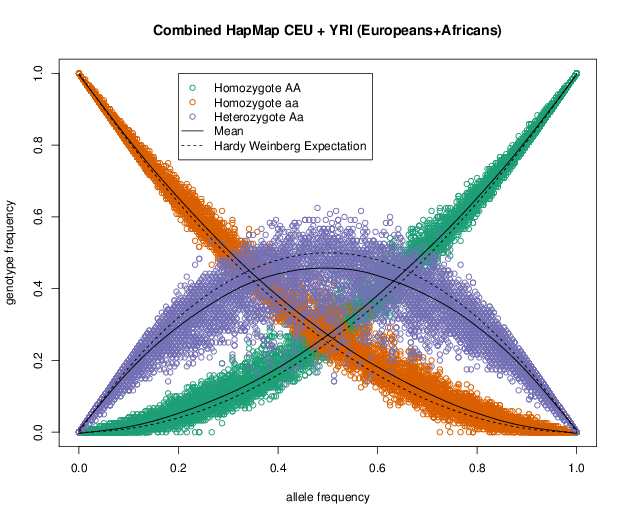
\includegraphics[width=0.5 \textwidth]{figures/CEU_YRI_together_HWE.png}
%\end{center}
%\caption{}
%\end{figure}


%figure/QT1.eps


\section{Allele sharing among related individuals and Identity by Descent}

All of the individuals in a population are related to each other by a giant
pedigree (family tree). For most pairs of individuals in a population these
relationships are very distant (i.e. distant cousins), while some individuals
will be more closely related (i.e. sibling/first cousins). All individuals of
are related to one another by varying levels of relatedness, or \emph{kinship}.
Related individuals can share alleles that have both descended from the shared
common ancestor. To be shared, these alleles must be inherited through all
meioses connecting the two individuals (e.g. surviving the $\nicefrac{1}{2}$
probability of segregation each meiosis). As closer relatives are separated by
fewer meioses, closer relatives share more alleles. In Figure
\ref{fig:IBD_cousins_chr_cartoon} we show the sharing of chromosomal regions
between two cousins. As we'll see, many population and quantitative genetic
concepts rely on how closely related individuals are, and thus we need some way
to quantify the degree of kinship among individuals. \\
\begin{figure}
\begin{center}
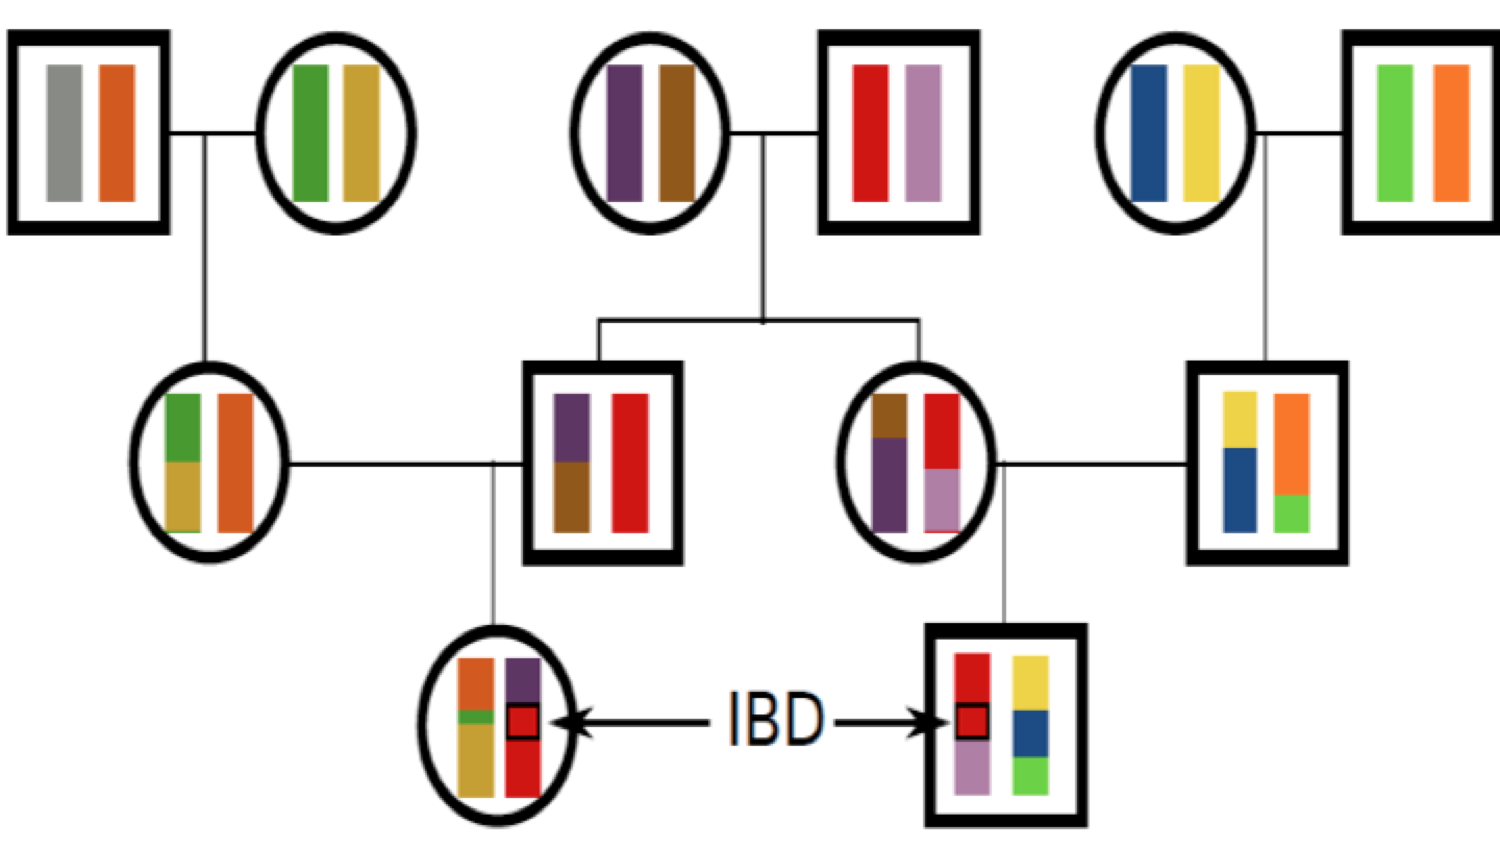
\includegraphics[width= 0.75 \textwidth]{figures/Cousins_IBD_chromo_cartoon.png}
\end{center}
\caption{First cousins sharing a stretch of chromosome identical by
  descent. The different grandparental diploid chromosomes are coloured so we
  can track them and recombinations between them across the
  generations. Notice that the identity by descent between the cousins persists for a long
stretch of chromosome due to the limited number of generations for
recombination.} \label{fig:IBD_cousins_chr_cartoon}  
\end{figure}

We will define two alleles to be identical by descent (IBD) if they are
identical due to transmission from a common ancestor in the past few generations\cite{cotterman:40,malecot:48}. For the moment,
we ignore mutation, and we will be more precise about what we mean by `past few
generations' later on. For example, parent and child share exactly one allele
identical by descent at a locus, assuming that the two parents of the child are
randomly mated individuals from the population. In Figure
\ref{fig:IBD_cousins_cartoon}, I show a pedigree demonstrating some
configurations of IBD. \\


One summary of how related two individuals are is the probability that our pair
of individuals share 0, 1, or 2 alleles identical by descent (see Figure
\ref{fig:IBD_0_1_2}). We denote these probabilities by $r_0$, $r_1$, and $r_2$
respectively. See Table \ref{table:IBDprobs} for some examples. We can also
interpret these probabilities as genome-wide averages. For example, on average,
full-sibs share zero alleles for a quarter of all of their autosomal loci.\\

\begin{marginfigure}
\begin{center}
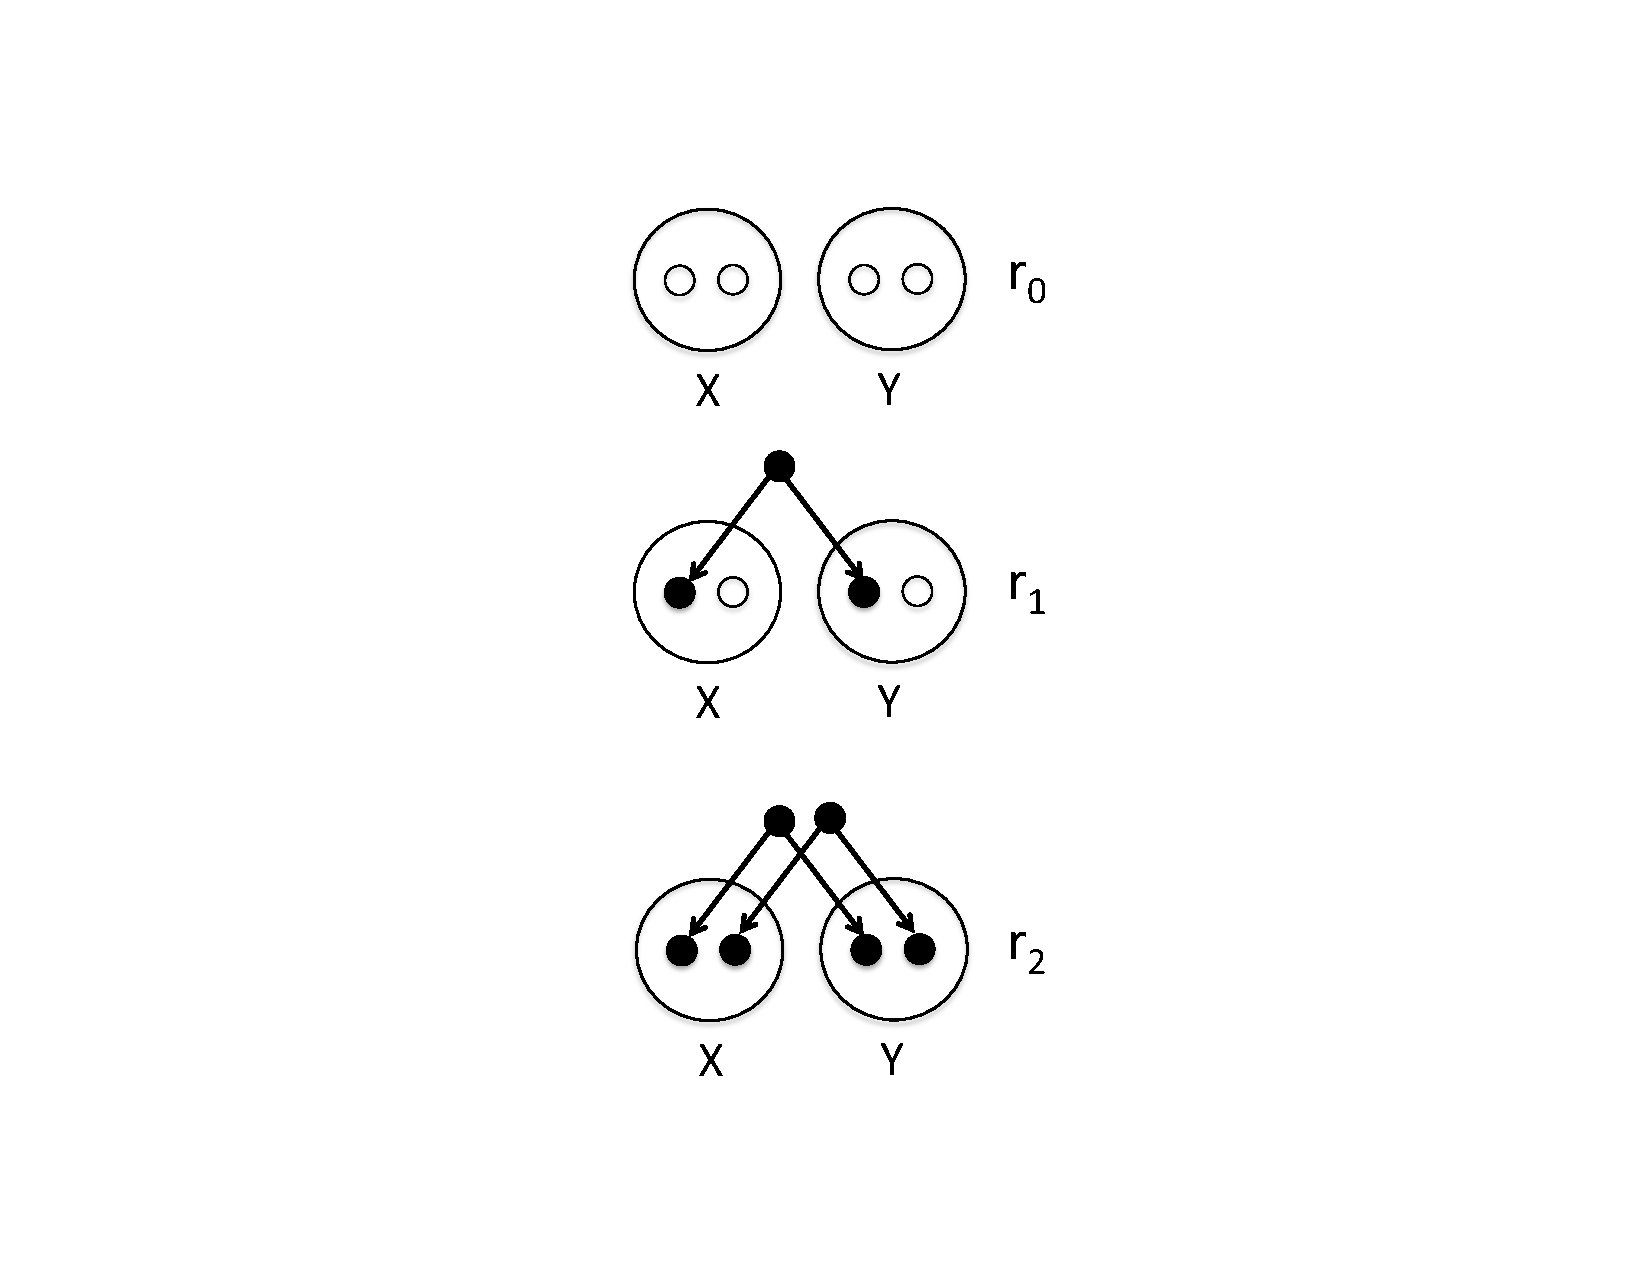
\includegraphics[width= 0.75 \textwidth]{figures/sharing_relatives/IBD_0_1_2.pdf} 
\end{center}
\caption{A diploid individuals (X and Y) sharing 0, 1, or 2 alleles IBD
  where lines show the sharing of alleles by descent (e.g. from a
  shared ancestor). } \label{fig:IBD_0_1_2}
\end{marginfigure}


One summary of relatedness that will be important is the probability that two
alleles picked at random, one from each of the two different individuals $i$
and $j$, are identical by descent. We call this quantity the \emph{coefficient
of kinship} of individuals $i$ and $j$, and denote it by $F_{ij}$. It is
calculated as

\begin{equation}
F_{ij}= 0 \times r_0 + \frac{1}{4} r_1  + \frac{1}{2} r_2. 
\label{eqn:coeffkinship}
\end{equation}
%
The coefficient of kinship will appear multiple times, in both our discussion of
inbreeding and in the context of phenotypic resemblance between relatives.\\


\begin{margintable}
\begin{center}
\begin{tabular}{ l c c c c}
\hline
Relationship (i,j)$^{*}$ & $r_0$ & $r_1$ & $r_2$ & $F_{ij}$\\
\hline
parent--child & 0 & 1 & 0 & \nicefrac{1}{4}\\
full siblings & \nicefrac{1}{4} & \nicefrac{1}{2} & \nicefrac{1}{4} & \nicefrac{1}{4}\\
Monzygotic twins  & 0 & 0 & 1  & \nicefrac{1}{2} \\
$1^{st}$ cousins & \nicefrac{3}{4} & \nicefrac{1}{4} & 0 & \nicefrac{1}{16}\\
\hline
\end{tabular}
\end{center}
\caption{Probability that two individuals of a given relationship share 0, 1, or 2 alleles
identical by descent on the autosomes. $^{*}$Assuming this is the only close relationship the pair shares. } % doesn't this implicitly assume an infinite population?
\label{table:IBDprobs}
\end{margintable}

\begin{question}
  What are $r_0$, $r_1$, and $r_2$ for $\nicefrac{1}{2}$ sibs? ($\nicefrac{1}{2}$ sibs share one
parent but not the other).
\end{question}

%Question 5. Consider a biallelic locus where allele 1 is at fre- quency p, and two individuals who have IBD allele sharing probabili- ties r0, r1, r2.
%What is the overall probability that these two individuals are both homozygous for allele 1?

Our $r$ coefficients are going to have a various uses. For example, they allow us
to calculate the probability of the genotypes of a pair of
relatives. Consider a biallelic locus where allele 1 is
at frequency $p$, and two individuals who have IBD allele sharing
probabilities $r_0$, $r_1$, $r_2$. What is the overall probability that these
two individuals are both homozygous for allele 1? Well that's
\begin{align}
  P(A_1 A_1) = &P(A_1 A_1 | \text{0 alleles IBD}) P(\text{0 alleles IBD})  \nonumber\\
  & + P(A_1 A_1 | \text{1 alleles IBD}) P(\text{1 alleles IBD})  \nonumber\\
  &+ P(A_1 A_1 | \text{2 alleles IBD}) P(\text{2 alleles IBD}) \\
\end{align}
in our $r_0$, $r_1$, $r_2$ notation
\begin{align}
  P(A_1 A_1) = P(A_1 A_1 | \text{0 alleles IBD}) r_0 + P(A_1 A_1 |
  \text{1 alleles IBD}) r_1 + P(A_1 A_1 | \text{2 alleles IBD}) r_2 \label{eqn:initial_relly_IBD_calc}
\end{align}
If our pair of relatives share $0$ alleles IBD, then the probability that
they are both homozygote is $P(A_1 A_1 |
\text{0 alleles IBD}) =p^2 \times p^2$, as all four alleles
represent independent draws from the population. If they share $1$
allele IBD, then this is of type $A_1$ with probability $p$, and then
the other non-IBD allele, in both relatives, also needs
to be $A_1$ which happens with probability $p^2$ so $P(A_1 A_1 |
\text{1 alleles IBD})=p \times p^2$. Finally our pair of relatives can
share two alleles IBD, in that case $P(A_1 A_1 | \text{2 alleles IBD})
= p^2$ as if one of our individuals is homozygote for the $A_1$ allele
both individuals will be. Putting this all together our
\eqref{eqn:initial_relly_IBD_calc} becomes 
\begin{equation}
P(A_1 A_2) = p^4 r_0 + p^3 r_1 + p^2 r_2 \label{eqn:IBD_relly_calc}
\end{equation}
Note that  for specific cases we could also calculate this by summing over the
genotypes of their shared ancestor was; however, that would be much more
involved and not as general as the form we have derived here.

We can write out terms like eq \eqref{eqn:IBD_relly_calc} for all of
the possible configurations of genotype
sharing/non-sharing between a pair of individuals. Based on this we can write down the expected number of
polymorphic sites where our individuals are observed to share 0, 1, or 2
alleles. There's a variety of ways to estimate the relationships among
individuals. 

\begin{question}
The genotype of our suspect in Question \ref{Q:CODIS} turns out to be 100/80 for
D16S539 and 70/80 at TH01. The suspect is not a match to the DNA
from the crime scene; however, they could be a sibling.

Calculate the joint probability of the genotype from the  crime and our
suspect:\\
{\bf A)} Assuming that they share no close relationship.\\

{\bf B)} Assuming that they are full sibs.\\

{\bf C)} Briefly explain your findings.  
  \end{question}

 \begin{marginfigure}
\begin{center}
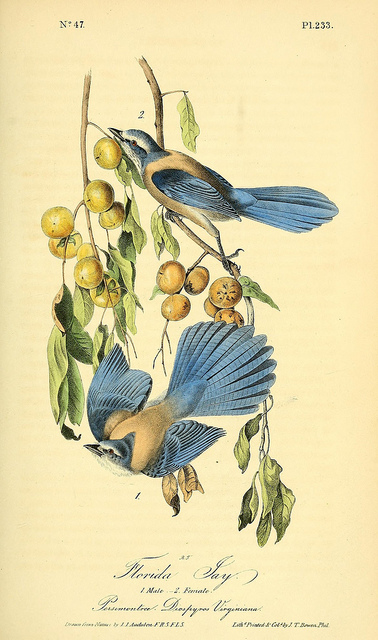
\includegraphics[width= \textwidth]{illustration_images/alleles_genotypes/Florida_scrub_jay/8576533889_3a131ffc4c_z.jpg}
\end{center}
\caption{Florida Scrub-Jays ({\it Aphelocoma coerulescens}). The birds of America : from drawings made in the United
  States and their territories. 1880. Audubon J.J.
} \label{fig:FSJ}  
\end{marginfigure}

  
An example of using allele sharing to identify relatives is offered by
the work on Nancy Chen. She has collected genotyping data from thousands of
Florida Scrub Jays at over ten thousand loci. These Jays live at the
Archbold field site, and have been carefully monitored for many
decades allowing the pedigree of many of the birds to be known.
Using these data she could estimate allele frequencies at each
locus. Then by equating the observed number of times that a pair of
individuals share $0$, $1$, or $2$ alleles to the theoretical
expectation she can estimate the probability of $r_0$, $r_1$, and
$r_2$ for each pair of birds. A plot of these are shown in Figure
\ref{fig:FSJ_IBD}, showing how well the estimates match those known
from the pedigree.

%\end{question}


\begin{figure}
\begin{center}
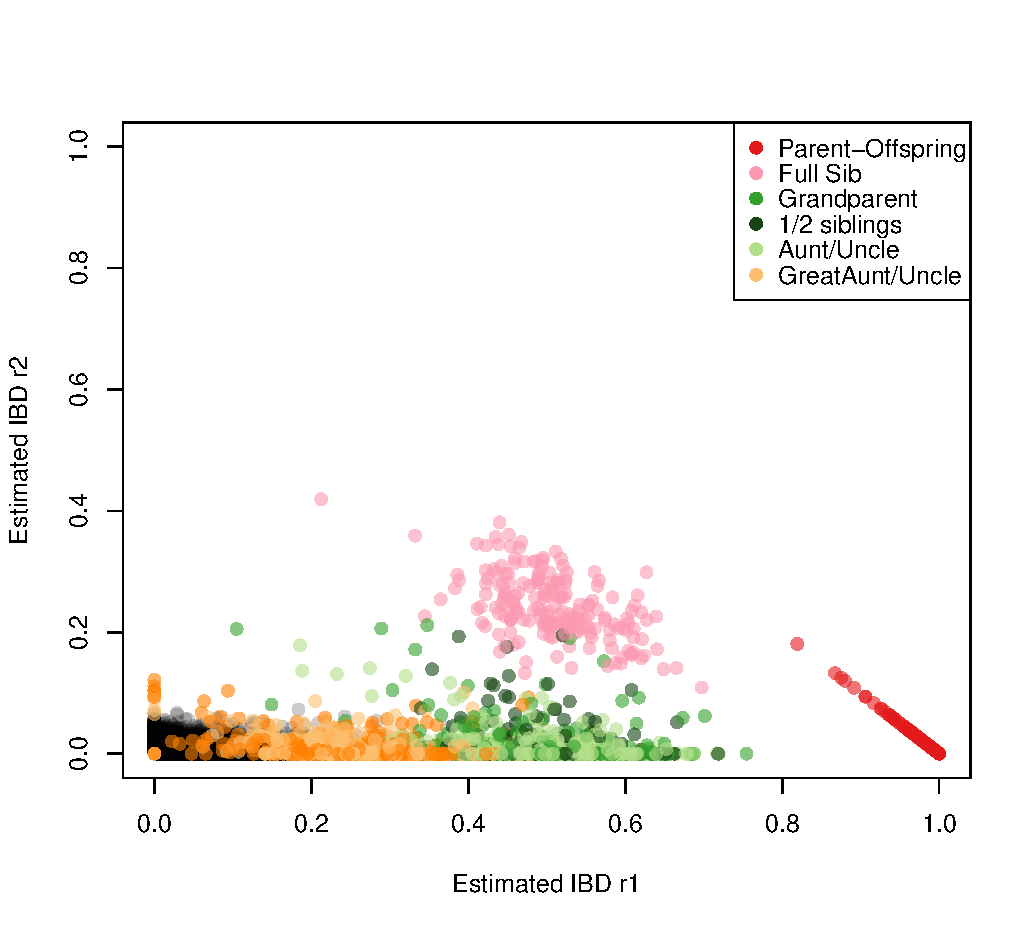
\includegraphics[width= \textwidth]{figures/FSJ_IBD.pdf}
\end{center}
\caption{} \label{fig:FSJ_IBD}  
\end{figure}


\subsection{Inbreeding}
We can define an inbred individual as an individual whose parents are
more closely related to each other than two random individuals drawn
from some reference population.  \\


\begin{figure}
\begin{center}
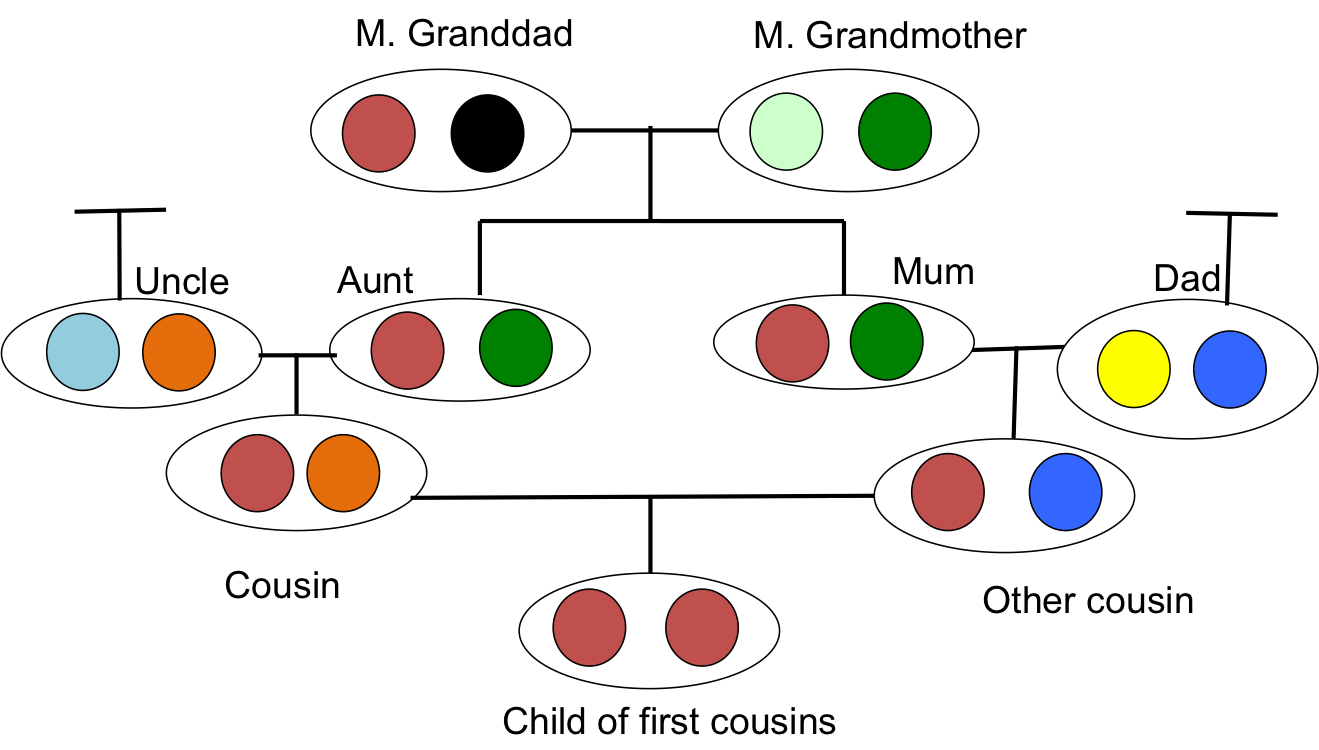
\includegraphics[width= 0.5 \textwidth]{figures/Child_first_cousins_Homozy_BD.png}
\end{center}
\caption{Alleles being transmitted through an inbred pedigree. The mum and the
  aunt share two alleles identical by descent (IBD). The cousins share one
  allele IBD. The offspring of first cousins is homozygous by
  descent at this locus.} \label{fig:IBD_cousins_cartoon}  
\end{figure}

When two related individuals produce an offspring, that individual can
receive two alleles that are identical by descent, i.e.\ they
can be homozygous by descent (sometimes termed autozygous), due to the
fact that they have two copies of an allele through different paths
through the pedigree.  This increased likelihood of being homozygous
relative to an outbred individual is the most obvious effect of
inbreeding. It is also the one that will be of most interest to us, as it
underlies a lot of our ideas about inbreeding depression and
population structure. For example, in Figure \ref{fig:IBD_cousins_cartoon} our
offspring of first cousins is homozygous by descent having received
the same IBD allele via two different routes around an inbreeding loop.\\

As the offspring receives a random allele from each parent ($i$ and $j$), the
probability that those two alleles are identical by descent is equal to the
kinship coefficient $F_{ij}$ of the two parents (Eqn.\ \ref{eqn:coeffkinship}). This follows from the fact that
the genotype of the offspring is made by sampling an allele at random from each
of our parents. % We will use IBD for identical by descent. \\ %% this was already defined above.

\begin{margintable}
\begin{center}
\begin{tabular}{ccc}
\hline
$f_{11}$ & $f_{12}$ & $f_{22}$ \\
\hline
$(1-F) p^2 + F p$ & $(1-F) 2pq$ & $(1-F) q^2 + F q$ \\
\hline
\end{tabular}
\end{center}
\caption{\textbf{Generalized Hardy--Weinberg}} \label{table:GeneralizedHWE}
\end{margintable}


The only way the offspring can be heterozygous ($A_1 A_2$) is if their two
alleles at a locus are not IBD (otherwise they would necessarily be
homozygous). Therefore, the probability that they are heterozygous is

\begin{equation}
(1-F) 2p q,
\label{eq:hetGenHW}
\end{equation}
%
where we have dropped the indices $i$ and $j$ for simplicity.  The offspring
can be homozygous for the $A_1$ allele in two different ways.  They can have
two non-IBD alleles that are not IBD but happen to be of the allelic type
$A_1$, or their two alleles can be IBD, such that they inherited allele $A_1$
by two different routes from the same ancestor. Thus, the probability that an
offspring is homozygous for $A_1$ is

\begin{equation}
(1-F) p^2 + F p.
\end{equation}
%
Therefore, the frequencies of the three possible genotypes can be written as given in
Table \ref{table:GeneralizedHWE}, which provides a generalization of the Hardy--Weinberg
proportions.\\


Note that the generalized Hardy--Weinberg proportions completely
specify the genotype probabilities, as there are two parameters ($p$ and $F$)
and two degrees of freedom (as $p$ and $q$ have to sum to one).
Therefore, any combination of genotype frequencies at a biallelic site
can be specified by a combination of $p$ and $F$.\\
\marginnote{
\begin{question}
The frequency of the $A_1$ allele is $p$ at a biallelic locus. Assume that our population is randomly mating and that the
genotype frequencies in the population follow from HW. We select two
individuals at random to mate from this population. We then mate the children
from this cross. What is the probability that the child from this full
sib-mating is
homozygous? 
\end{question}
}
\subsection{Calculating inbreeding coefficients from data}

If the observed heterozygosity in a population is $H_O$, and we assume that the
generalized Hardy--Weinberg proportions hold, we can set $H_O$ equal to
$f_{12}$, and solve Eq.\ \eqref{eq:hetGenHW} for $F$ to obtain an estimate of
the inbreeding coefficient as

\begin{equation}
\hat{F} = 1-\frac{f_{12}}{2pq} = \frac{2pq - f_{12}}{2pq}.
\label{eqn:Fhat}
\end{equation}

\marginnote{
\begin{question} 
  Suppose the following genotype frequencies were observed for at an esterase locus in a population of \emph{Drosophila} (A denotes the ``fast" allele and B denotes the ``slow" allele): 
\begin{center}
\begin{tabular}{ccc}
\hline
AA &	AB &	BB\\
\hline
0.6 &	0.2 &	0.2\\
\end{tabular}
\end{center}
What is the estimate of the inbreeding coefficient at the esterase locus?
\end{question}
}

As before, $p$ is the frequency of allele $A_{1}$ in the population. This can
be rewritten in terms of the observed heterozygosity ($H_O$) and the
heterozygosity expected in the absence of inbreeding, $H_E=2pq$, as
\begin{equation}
\hat{F} = \frac{H_E-H_O}{H_E} = 1 - \frac{H_O}{H_E}.
\label{eqn:FhatHO}
\end{equation}
Hence, $\hat{F}$ quantifies the deviation due to inbreeding of the observed heterozygosity from the one expected under random mating, relative to the latter.
If we have multiple loci, we can replace $H_O$ and $H_E$ by their means
over loci, $\bar{H}_O$ and $\bar{H}_E$, respectively. Note that, in principle, we could also calculate $F$ for each individual locus first, and then take the average across loci. However, this procedure is more prone to introducing a bias if sample sizes vary across loci, which is not unlikely when we are dealing with real data.\\

%{\bf Q}\arabic{Question} \refstepcounter{Question} 

%==Phenotypic resemblance between relatives ==
%<source-file filename="Quantative_traits.tex" display="Quantative_traits.wrapped.latexml.xhtml">

%==Phenotypic resemblance between relatives ==
%<source-file filename="Quantative_traits.tex" display="Quantative_traits.wrapped.latexml.xhtml">


\section{Summarizing population structure}
\newthought{Individuals rarely mate complete at random}, your parents
weren't two Bilateria plucked at random from the tree of
life. Even within species, there's often geographically-restricted
mating among individuals. Individuals tend to mate with individuals
from the same, or closely related sets of populations. This form of
non-random mating is called population structure and can have profound
effects on the distribution of genetic variation within and among
natural populations.  

\subsection{Inbreeding as a summary of population structure.}
It turns out that statements about inbreeding represent one natural
way way to summarize population structure. We defined inbreeding as having parents that are more closely related to each other than two individuals drawn at random from some reference population. The question that naturally arises is: Which reference population should we use? While I might not look inbred in
comparison to allele frequencies in the United Kingdom (UK), where I am from, my
parents certainly are not two individuals drawn at random from the
world-wide population. If we estimated my inbreeding coefficient $F$ using allele frequencies
within the UK, it would 
be close to zero, but would likely be larger if we used world-wide
frequencies. This is because there is a somewhat lower level of
expected heterozygosity within the UK than in the human population across the world as a whole.\\

\citeauthor{Wright:43}\cite{Wright:43,Wright:49} developed a set of `F-statistics' (also called `fixation
indices') that formalize the idea of inbreeding with respect to different
levels of population structure. See Figure \ref{fig:FST_pig} for a schematic
diagram. Wright defined $F_{\mathrm{XY}}$ as the correlation between random
gametes, drawn from the same level $X$, relative to level $Y$. We will return
to why $F$-statistics are statements about correlations between alleles in just
a moment. One commonly used $F$-statistic is $\fis$, which is the inbreeding
coefficient between an individual ($I$) and the subpopulation ($S$). Consider a
single locus, where in a subpopulation ($S$) a fraction $H_I=f_{12}$ of
individuals are heterozygous.  In this subpopulation, let the frequency of
allele $A_1$ be $p_S$, such that the expected heterozygosity under random
mating is $H_S = 2 p_S (1 - p_S)$. We will write $\fis$ as
\begin{marginfigure}
\begin{center}
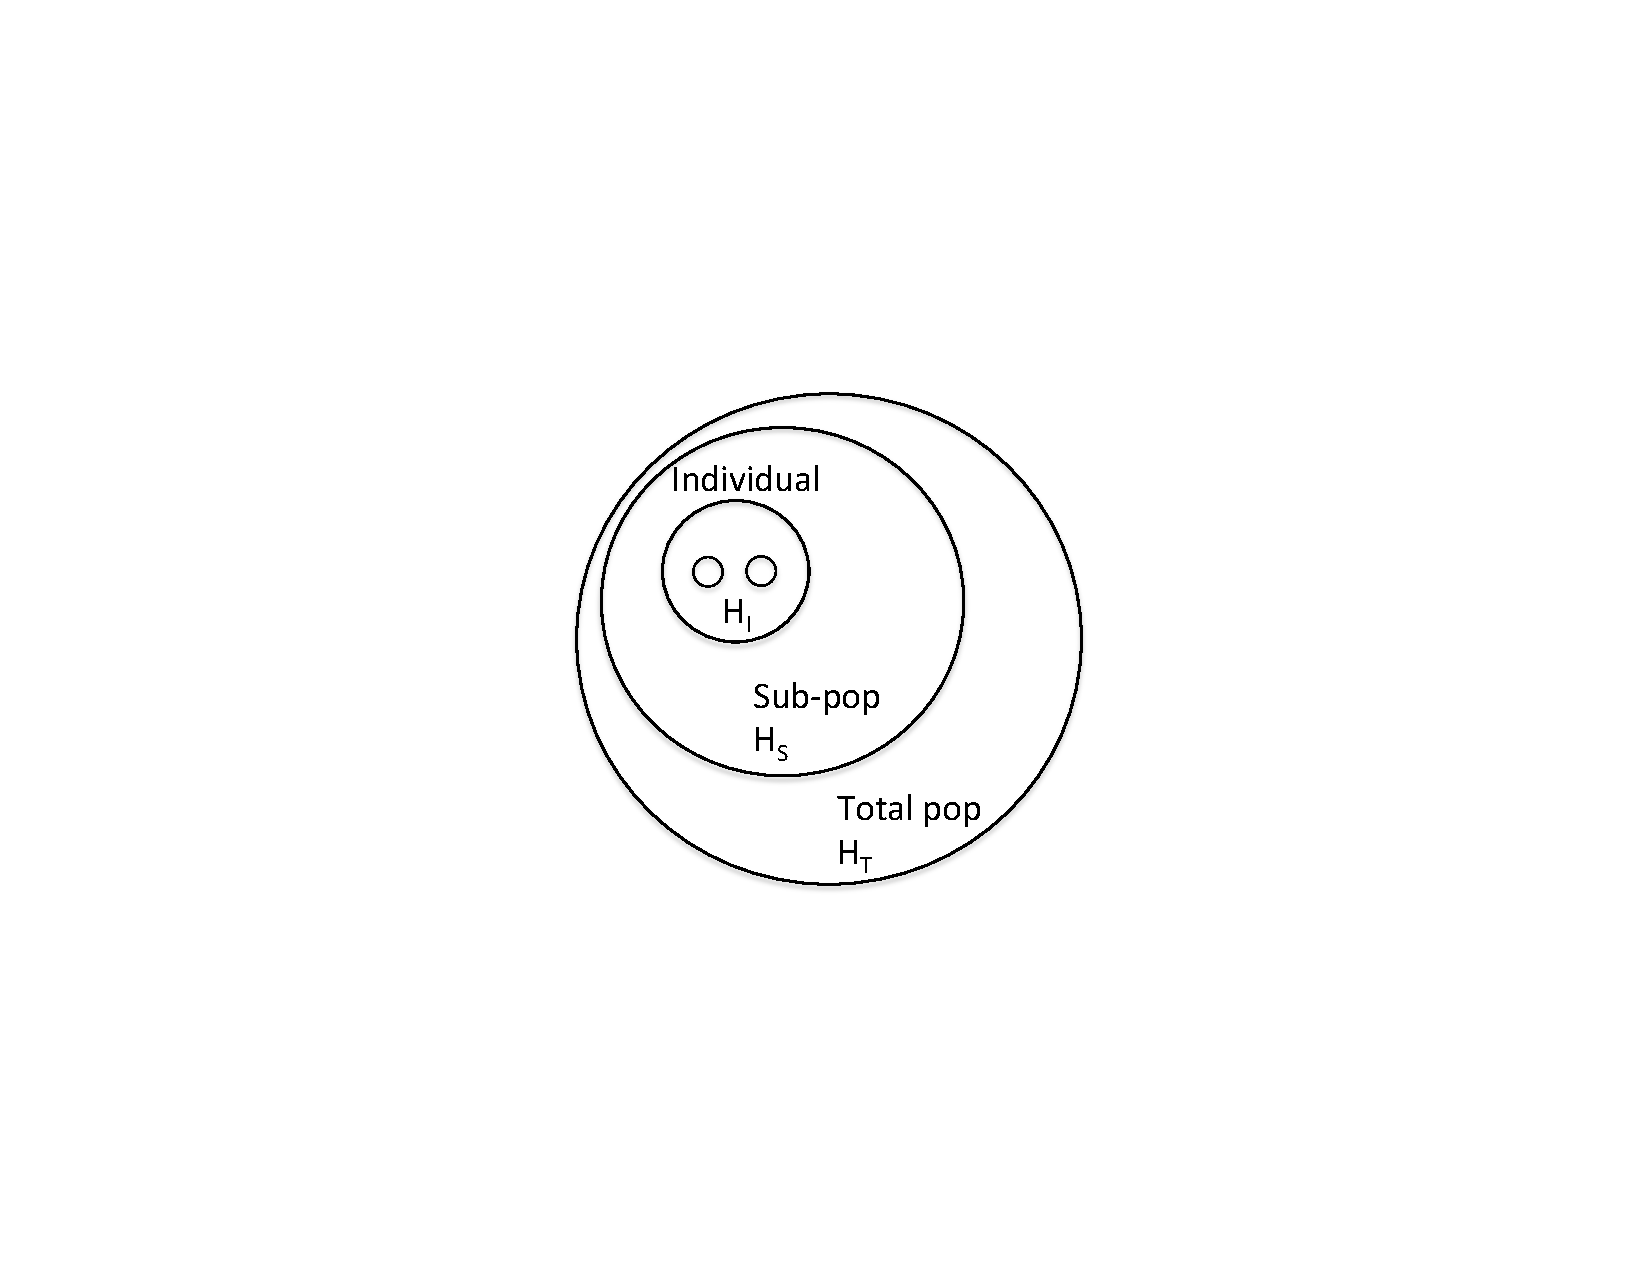
\includegraphics{figures/Pop_struct/FST_hierarchy.pdf}  %[width= \marginwidth]
\end{center}
\caption{The hierarchical nature of F-statistics. The two dots within an individual represent the two
  alleles at a locus for an individual $I$. We can compare the heterozygosity on individuals ($H_I$), to that found
by randomly drawing alleles from the sub-population (S),
to that found in the total population (T). } \label{fig:FST_pig}  
\end{marginfigure}
\begin{equation}
\fis = 1-\frac{H_I}{H_S}= 1-\frac{f_{12}}{2p_Sq_S},
\label{eqn:FIS}
\end{equation}
a direct analog of eqn. \ref{eqn:Fhat}. Hence, $\fis$ is the relative difference between observed and expected heterozygosity due to a deviation from random mating within the subpopulation. We could also compare the observed
heterozygosity in individuals ($H_I$) to that expected in the total
population, $H_T$. If the frequency of allele $A_1$ in the total
population is $p_T$, then we can write $\fit$ as
\begin{equation}
\fit =1-\frac{H_I}{H_T}= 1-\frac{f_{12}}{2p_Tq_T},
\label{eqn:FIT}
\end{equation}
which compares heterozygosity in individuals to that expected in the
total population. As a simple extension of this, we could imagine
comparing the expected heterozygosity in the subpopulation ($H_S$) to
that expected in the total population $H_T$, via $\fst$:
\begin{equation}
\fst = 1-\frac{H_S}{H_T}=1-\frac{2p_Sq_S}{2p_Tq_T} \label{eqn:FST}.
\end{equation}
If the total population contains the subpopulation then
 $2p_Sq_S \leq
2p_Tq_T$, and so $\fis \leq \fit$ and $\fst \geq 0$. We can
relate the three $F$-statistics to each other as
\begin{equation}
(1-\fit) =\frac{H_I}{H_S} \frac{H_S}{H_T}=(1-\fis)(1-\fst).
\label{eqn:F_relationships}
\end{equation}
Hence, the reduction in heterozygosity within individuals compared to that expected
in the total population can be decomposed to the reduction in
heterozygosity of individuals compared to the subpopulation, and the reduction in
heterozygosity from the total population to that in the subpopulation.\\
%n, as we will seebelow, due to the Wahlund effect (to be added)

If we want a summary of
population structure across multiple subpopulations, we can average $H_I$
and/or $H_S$ across populations, and use a $p_T$ calculated by
averaging $p_S$ across subpopulations (or our samples from sub-populations). For example, the average $\fst$ across $K$ subpopulations (sampled with equal effort) is
\begin{equation}
	\fst = 1 - \frac{\bar{H}_{S}}{H_T},
\end{equation}
where $\bar{H}_S = \nicefrac{1}{K} \sum_{i = 1}^{K} H_{S}^{(i)}$, and
$H_{S}^{(i)} = 2 p_{i} q_{i}$ is the expected heterozygosity in subpopulation
$i$.  Furthermore, if we have multiple sites, we can replace $H_I$, $H_S$, and
$H_T$ with their averages across loci (as above). \\


\begin{marginfigure}
\begin{center}
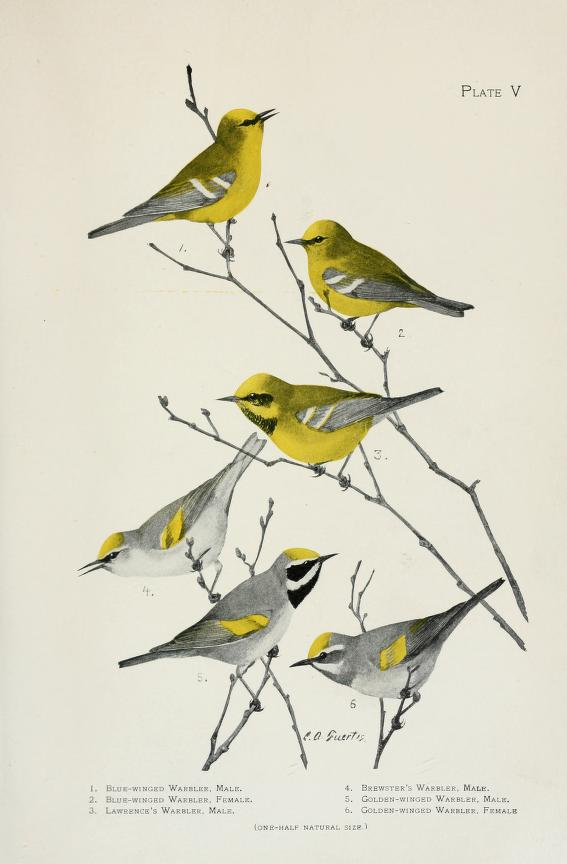
\includegraphics[width = \textwidth]{illustration_images/alleles_genotypes/blue_golden_winged_warblers/The_warblers_of_North_America_6309257188.jpg}  %[width= \marginwidth]
\end{center}
\caption{The warblers of North America. Chapman, F.M. 1907.} \label{fig:blue_golden_warblers}  
\end{marginfigure}

As an example of comparing a genome-wide estimate of $F_{ST}$ to that
at individual loci we can look at some data from blue- and
golden-winged warblers ({\it Vermivora cyanoptera} and {\it
  V. chrysoptera} 1-2 \& 5-6 o, Figure  \ref{fig:blue_golden_warblers}). These two species are spead across eastern
Northern America, with the golden-winged warbler having a smaller, more
northernly range. They're quite different in terms of plumage, but
have long been known to have similar songs and ecologies. The two species
hybridize readily in the wild; in fact two other previously-recognized species, Brewster's
and Lawrence’s warbler (4 \& 3 in \ref{fig:blue_golden_warblers}), actually just being hybirds between theses two species. 
The golden-winged warbler is listed as `threatened' under the Canadian
endangered species act, its habitat is under pressure for human activity
and hybrization with the blue warbler as it moves north also poses a
significant issue. \citeauthor{Toews:16} investigated the population
genomics of these warblers, sequencing ten golden- and ten blue-winged
warblers. They found very low divergence among these species, with a
genome-wide $F_{ST}=0.0045$. In Figure \ref{fig:warbler_FST}, per SNP
$F_{ST}$ is averaged in $2000$bp windows moving along the genome. 
\begin{figure*}
\begin{center}
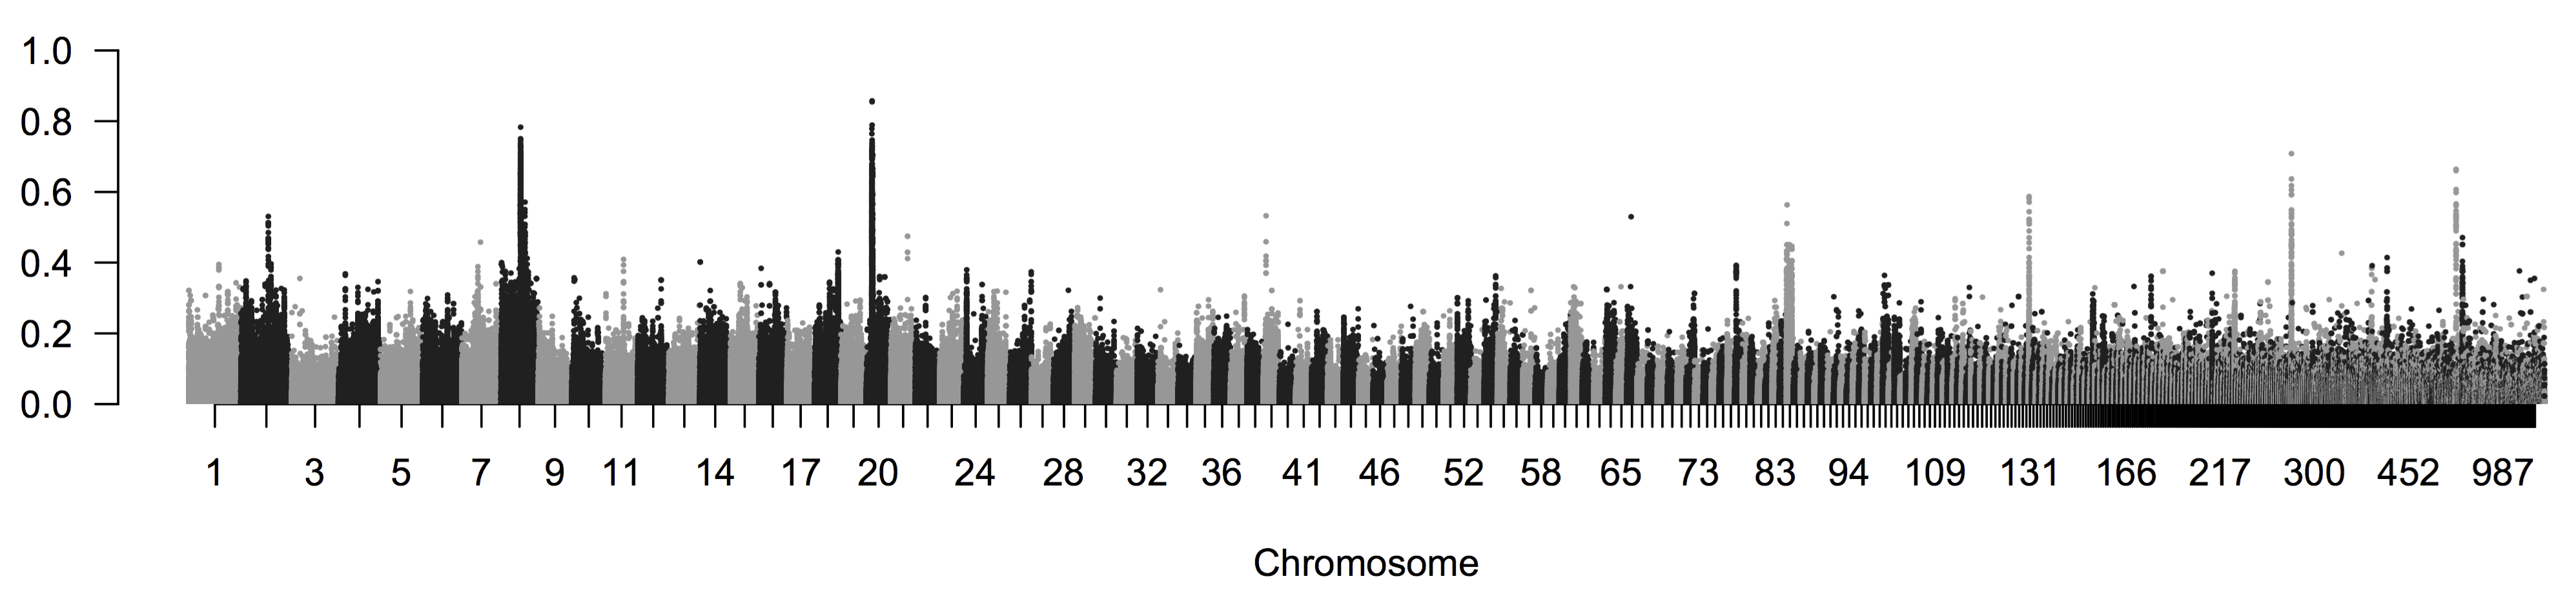
\includegraphics[width = 0.8 \textwidth]{Journal_figs/alleles_genotypes/blue_golden_winged_warblers/GW_FST_warblers.png}  %[width= \marginwidth]
\end{center}
\caption{Thanks to David Toews for the figure. } \label{fig:warbler_FST}  
\end{figure*}
The average is very low, but some regions of very high $F_{ST}$ stand
out. Nearly all of these regions correspond to large allele frequency
difference at loci in, or close, to genes known to be involved in
plumage colouration difference in other birds.  
To illustrate these frequency differences \citeauthor{Toews:16}
genotyped a SNP in each of this high-$F_{ST}$ regions. Here's their
geotyping counts from the SNP in the {\it Wnt}
region, a key regulatory gene involved in feather development:
\begin{center}
\begin{tabular}{ l c c c}
Species & 11 & 12 & 22\\
\hline
Blue-winged & 2 & 21 & 31\\
Golden-winged & 48 & 12 & 1\\
\hline   
\end{tabular}
\end{center}

\begin{question}
With reference to the table of {\it Wnt}-allele frequency:\\
{\bf A)} Calculate $F_{IS}$ in blue-winged warblers.\\
{\bf B)} Calculate $F_{ST}$ for the sub-population of blue-winged
warblers compared to the combined sample.\\
{ \bf C)} Calculate $F_{ST}$ for both sub-populations.
\end{question}

\paragraph{Interpretations of F-statistics}

Let us now return to Wright's definition of the $F$-statistics as correlations
between random gametes, drawn from the same level $X$, relative to level $Y$.
Without loss of generality, we may think about $X$ as individuals and $S$ as
the subpopulation.  Rewriting $\fis$ in terms of the observed homozygote
frequencies ($f_{11}$, $f_{22}$) and expected homozygosities ($p_{S}^2$,
$q_{S}^2$) we find
\begin{equation}
\fis = \frac{2p_Sq_S - f_{12}}{2p_Sq_S} = \frac{f_{11}+f_{22} -
p_S^2 - q_S^2}{2p_Sq_S},
\label{eqn:Fascorr}
\end{equation}
using the fact that $p^2+2pq+q^2=1$, and $f_{12} = 1 - f_{11} - f_{12}$. The
form of eqn.\ (\ref{eqn:Fascorr}) reveals that $\fis$ is the covariance between
pairs of alleles found in an individual, divided by the expected variance under
binomial sampling. Thus, $F$-statistics can be understood as the correlation
between alleles drawn from a population (or an individual) above that expected
by chance (i.e.\ drawing alleles sampled at random from some broader
population).\\

We can also interpret $F$-statistics as proportions of variance explained by
different levels of population structure. To see this, let us think about $\fst$ averaged over $K$
subpopulations, whose frequencies are $p_1,\dots,p_K$. The
frequency in the total population is $p_T=\bar{p} = \nicefrac{1}{K} \sum_{i=1}^K p_i$.
Then, we can
write
\begin{equation}
\fst = \frac{2 \bar{p}\bar{q} - \frac{1}{K}\sum_{i=1}^K 2p_iq_i }{2
\bar{p}\bar{q}} = \frac{ \left(\frac{1}{K} \sum_{i=1}^K p_i^2 +
\frac{1}{K} \sum_{i=1}^K q_i^2 \right) -  \bar{p}^2-\bar{q}^2 }{2
\bar{p}\bar{q}} = \frac{\mathrm{Var}(p_i)}{\mathrm{Var}(\bar{p})},
\label{eqn:F_as_propvar}
\end{equation}
which shows that $\fst$ is the proportion of the variance explained by the
subpopulation labels.

\subsection{Other approaches to population structure}

There is a broad spectrum of methods to describe patterns of population
structure in population genetic datasets. We'll briefly discuss two
broad-classes of methods that appear often in the literature: assignment
methods and principal components analysis.

\subsection{Assignment Methods}

Here we'll describe a simple probabilistic assignment to find the
probability that an individual of unknown population comes from one of
$K$ predefined populations. For example, there are three broad populations
of common chimpanzee ({\it Pan troglodytes}) in Africa: western,
central, and eastern. Imagine that we have a chimpanzee, whose
population of origin is unknown (e.g. it's from an illegal private
collection). If we have genotyped a set of unlinked markers from a panel
of individuals representative of these populations, we can calculate
the probability that our chimp comes from each of these populations. \\   

We'll then briefly explain how to extend this idea
to cluster a set of individuals into $K$ initially unknown populations. This
method is a simplified version of what population genetics
clustering algorithms such as STRUCTURE and ADMIXTURE do. \cite{pritchard:00,alexander:09} 

\paragraph{A simple assignment method}

We have genotype data from unlinked $S$ biallelic loci for $K$ populations. The
allele frequency of allele $A_1$ at locus $l$ in population $k$ is denoted by
$p_{k,l}$, so that the allele frequencies in population 1 are $p_{1,1},\cdots
p_{1,L}$ and population 2 are $p_{2,1},\cdots p_{2,L}$ and so on. 

You type a new individual from an unknown population at these $L$ loci. This individual's genotype at locus $l$ is $g_l$, where $g_l$ denotes the number of copies of allele $A_1$ this individual carries at this locus ($g_l=0,1,2$). 

The probability of this individual's genotype at locus $l$ conditional on coming from population $k$, i.e. their alleles being a random HW draw from population $k$, is 
\begin{equation}
  P(g_l | \textrm{pop k}) =
  \begin{cases}
(1-p_{k,l})^2  & g_l=0 \\
2 p_{k,l} (1-p_{k,l}) & g_l=1\\
p_{k,l}^2  & g_l=2
\end{cases}
\end{equation}

Assuming that the loci are independent, the probability of individual's genotypes conditional on them coming from population $k$ is 
\begin{equation}
P(\textrm{ind.} | \textrm{pop k})  = \prod_{l=1}^S P(g_l | \textrm{pop k}) \label{eqn_assignment}
\end{equation}

% TODO: deleted "new" in bayes -- this is confusing I think for students
We wish to know the probability that this new individual comes from population
$k$, i.e. $P(\textrm{pop k} | \textrm{ind.})$. We can obtain this through Bayes
rule 

\begin{equation}
 P(\textrm{pop k} | \textrm{ind.})  = \frac{P(\textrm{ind.} | \textrm{pop k}) P(\textrm{pop k})}{P(\textrm{ind.})}
\end{equation}
where 
\begin{equation}
P(\textrm{ind.}) = \sum_{k=1}^K  P(\textrm{ind.} | \textrm{pop k}) P(\textrm{pop k})
\end{equation}
is the normalizing constant. We interpret $P(\textrm{pop k})$ as the
prior probability of the individual coming from population $k$, unless
we have some other prior knowledge we will assume that the new individual has a equal probability of coming from each population $P(\textrm{pop k})=\nicefrac{1}{K}$.  

We interpret 
\begin{equation}
 P(\textrm{pop k} | \textrm{ind.})
\end{equation}
as the posterior probability that our new individual comes from each of our $1,\cdots, K$ populations.

More sophisticated versions of this are now used to allow for hybrids,
e.g, we can have a proportion $q_k$ of our individual's genome come
from population $k$ and estimate the set of $q_k$'s.

%{\bf Q}\arabic{Question} \refstepcounter{Question}  
\begin{question} 

Returning to our chimp example, imagine that we have genotyped a set of
individuals from the Western and Eastern populations at two SNPs (we'll ignore
the central population to keep things simpler).  The frequency of the capital
allele at two SNPs ($A/a$ and $B/b$) is given by

\begin{center}
\begin{tabular}{|ccc|}
\hline
Population & locus A & locus B \\
\hline
Western & $0.1$ & $0.85$ \\
Eastern  & $0.95$ & $0.2$ \\
%Eastern & $0.5$ & $0.5$ \\
\hline
\end{tabular}
\end{center}
%
{\bf A)} Our individual, whose origin is unknown, has the genotype $AA$ at the
first locus and $bb$ at the second. What is the posterior probability that our
individual comes from the Western population versus Eastern chimp population?\\[1 em]
%
{\bf B)} Lets assume that with probability $q_W$ our individual draws an allele
from the Western population and that with probability $q_C=1-q_W$ they draw an
allele from the Eastern population. What is the probability of our individual's
genotype given $q_C$? \\

{\bf Optional} You could plot this probability as a function of $q_W$. How does 
your plot change if our individual is heterozygote at both loci?
\end{question} 

\paragraph{Clustering based on assignment methods}

While it is great to be able to assign our individuals to particular
population, these ideas can be pushed to learn about how best to describe our
genotype data in terms of discrete populations without assigning any of our
individuals to populations {\it a priori}.  We wish to cluster our individuals
into $K$ unknown populations. We begin by assigning our individuals at random
to these $K$ populations. 
\begin{enumerate}
\item Given these assignments we estimate the allele frequencies at all of our loci in each population. 
\item Given these allele frequencies we chose to reassign each individual to a population $k$ with a probability given by eqn. ($\ref{eqn_assignment}$).
\end{enumerate}
We iterate steps 1 and 2 for many iterations (technically, this approach is known as \emph{Gibbs Sampling}). If the data is
sufficiently informative the assignments and allele frequencies will
quickly converge on a set of likely population assignments and allele
frequencies for these populations. 

To do this in a full Bayesian scheme we need to place priors on the allele
frequencies (for example, one could use a beta distribution prior). Technically
we are using this is the joint posterior of our allele frequencies and
assignments. Programs like STRUCTURE, use this type of algorithm to
cluster the individuals in an ``unsupervised'' manner (i.e. they work
out how to assign individuals to unknown set of populations).  See Figure \ref{fig:chimp_structure} for an example of
Becquet {\it et al}  using STRUCTURE to determine the population structure of chimpanzees. 

\begin{figure}
% TODO: MISSING FIGURE
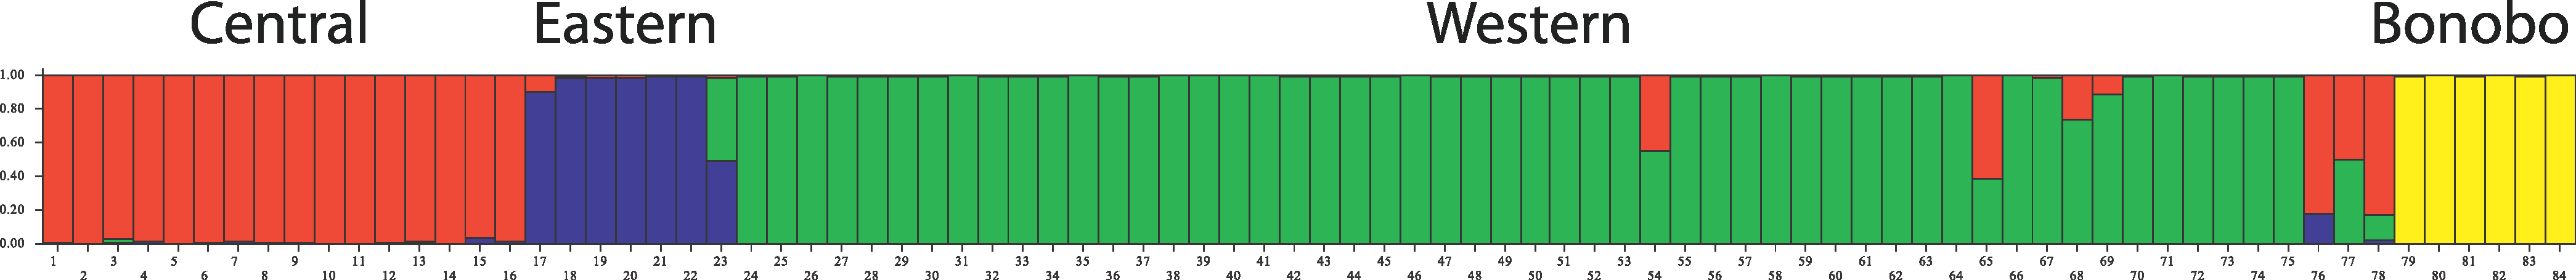
\includegraphics[width= \textwidth, height = 0.12 \textheight]{figures/Becquet_et_al_STRUCTURE_journal_pgen_0030066_g001.png}
\caption{
Becquet {\it et al.} (PLOS Genetics 2007) genotyped 78 common chimpanzee and 6 bonobo at
over 300 polymorphic markers (in this case microsatellites, a type of
multiallelic marker). They ran STRUCTURE to cluster the individuals
using these data into $K=4$
populations. In the above figure they show each individual as a
vertical bar divided into four colours depicting the estimate of the fraction
of ancestry that each individual draws from each of the four
estimated populations. We can see that these four colours/populations correspond to: Red, central; blue, eastern; green,
western; yellow, bonobo.  In their caption of this figure they say:  
{\it ``STRUCTURE Analysis, Blinded to Population Labels, Recapitulates the Reported Population Structure of the Chimpanzees
Individuals 76–-78 are reported hybrids. Only two individuals with a
$>5\%$ proportion of ancestry in more than one inferred cluster are wild
born: number 54 and number 17.''}} \label{fig:chimp_structure} % http://journals.plos.org/plosgenetics/article?id=10.1371%2Fjournal.pgen.0030066
%=======
%Individuals 76–78 are reported hybrids. Only two individuals with a $>5\%$ proportion of ancestry in more than one inferred cluster are wild born: number 54 and number 17. Red, central; blue, eastern; green, western; yellow, bonobo.''}
\end{figure}

\subsection{Principal components analysis}
Principal component analysis (PCA) is a common statistical approach to visualize  high dimensional data, and used by many fields. The idea of PCA is to give a location to  of each individual data-point on each of a small number principal component axes. These PC axes are chosen to reflect major axes of variation in the data,
  with the first PC being that which explains largest variance, the second the second most, and so on. The use of PCA in population genetics was
pioneered by Cavalli-Sforza and colleagues and With large genotyping datasets PCA has made come back. \cite{menozzi:78,patterson:06}
% TODO: citations.
 
Consider a dataset consisting of N individuals at $S$ biallelic SNPs. The
$i^{th}$ individual's genotype data at locus $\ell$ takes a value
$g_{i,\ell}=0,1,\; \text{or} \; 2$ (corresponding to the number of copies of
allele $A_1$ an individual carries at this SNP). We can think of this as a $N
\times S$ matrix (where usually $N \ll S$). 

Denoting the sample mean allele frequency at SNP $\ell$ by $p_{\ell}$ it's
common to standardize the genotype in the following way \begin{equation}
\frac{g_{i,\ell} - 2 p_{\ell}}{\sqrt{p_{\ell}(1-p_{\ell})}} \end{equation} i.e.
at each SNP we center the genotypes by subtracting the mean genotype
($2\epsilon_{\ell}$) and divide through by the expected variance assuming that
alleles are sampled binomially from the mean frequency ($\sqrt{p_{\ell}
  (1-p_{\ell})}$). Doing this to all of our genotypes we form a data matrix (of
  dimension $N \times S$). We can then perform principal components analysis of
  this data matrix to uncover the major axes of genotype variance in our
  sample. Figure \ref{fig:chimp_PCA} shows a PCA from Becquet \emph{et al.}
  (2007) using the same chimpanzee data as in Figure \ref{fig:chimp_structure}.

It is worth taking a moment to delve further into what we are doing
here. There's a number of equivalent ways to thinking about what PCA
is doing, one of these is to think that when we do PCA we are building the individual by individual
covariance matrix and performing eigenvalue decomposition of this
matrix (with the eigenvectors giving the PC).  This individual by individual covariance matrix has entries
the $(i,~j)^{th}$ entry given by
\begin{equation}
\sum_{\ell=1}^S \frac{(g_{i,\ell} - 2p_{\ell})(g_{j,\ell} - 2p_{\ell})}{p_{\ell}(1-p_{\ell})}
\end{equation}
note that this is the covariance, is very similar to those we
encountered in discussing $F$-statistics as correlations (equation
\eqref{eqn:Fascorr}), expect now we are asking about the allelic covariance
between two individuals above that expected if they were both drawn
from the total sample at random (rather than the covariance of alleles
within a single individual). So by performing PCA on the data we are
learning about the major (orthogonal) axes of the kinship matrix.    

\begin{figure}
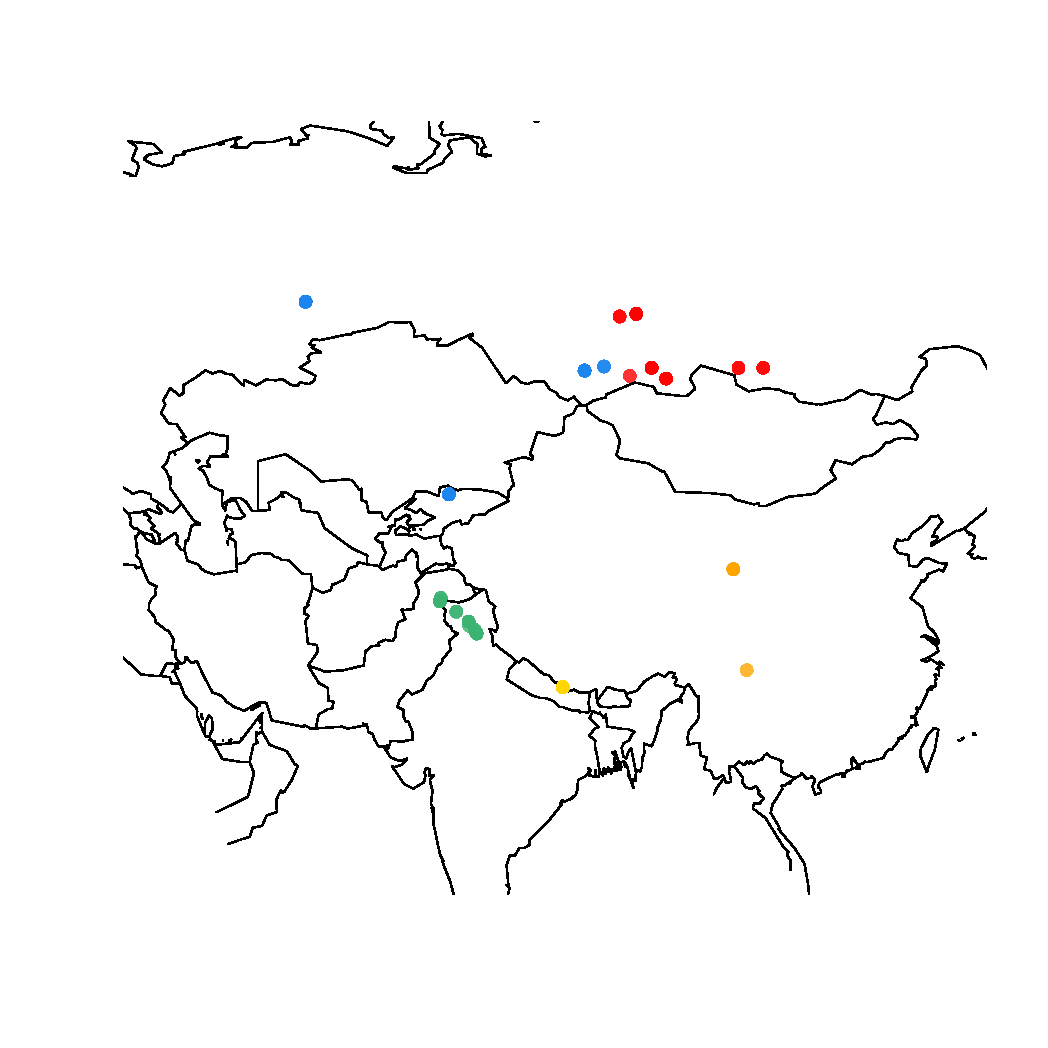
\includegraphics[width=
  0.5 \textwidth]{figures/warbler_PCA_figs/warbler_geo_map.pdf}
    \caption{  }
\label{fig:warbler_geo}
\end{figure}


\begin{figure}
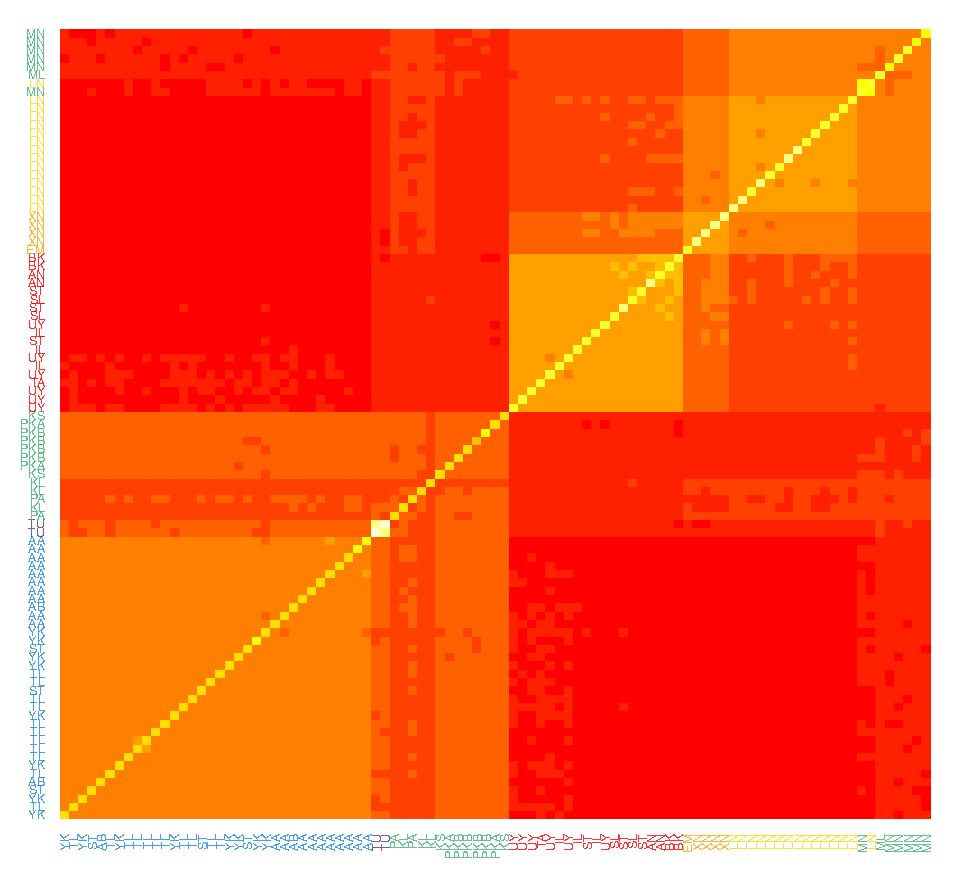
\includegraphics[width=
  0.75 \textwidth]{figures/warbler_PCA_figs/warbler_heatmap.pdf}
    \caption{  }
\label{fig:warbler_heat}
\end{figure}

\begin{figure}
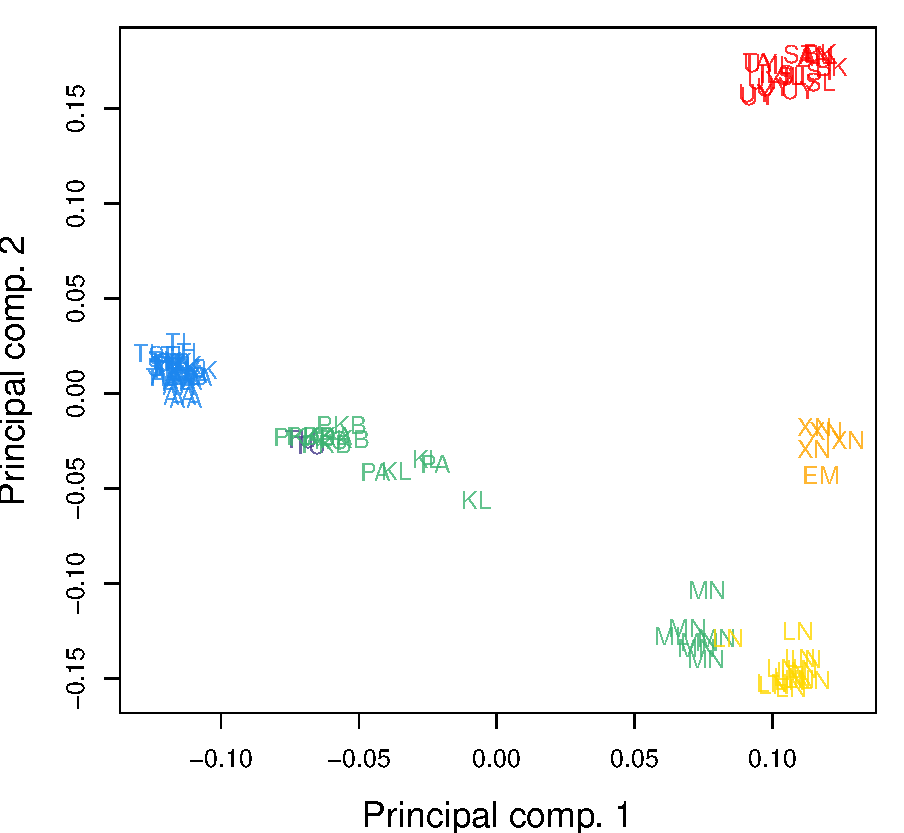
\includegraphics[width=
  0.75 \textwidth]{figures/warbler_PCA_figs/warbler_PCAmap.pdf}
    \caption{  }
\label{fig:warbler_PCA}
\end{figure}

% \begin{figure}
% % TODO: MISSING FIGURE
% 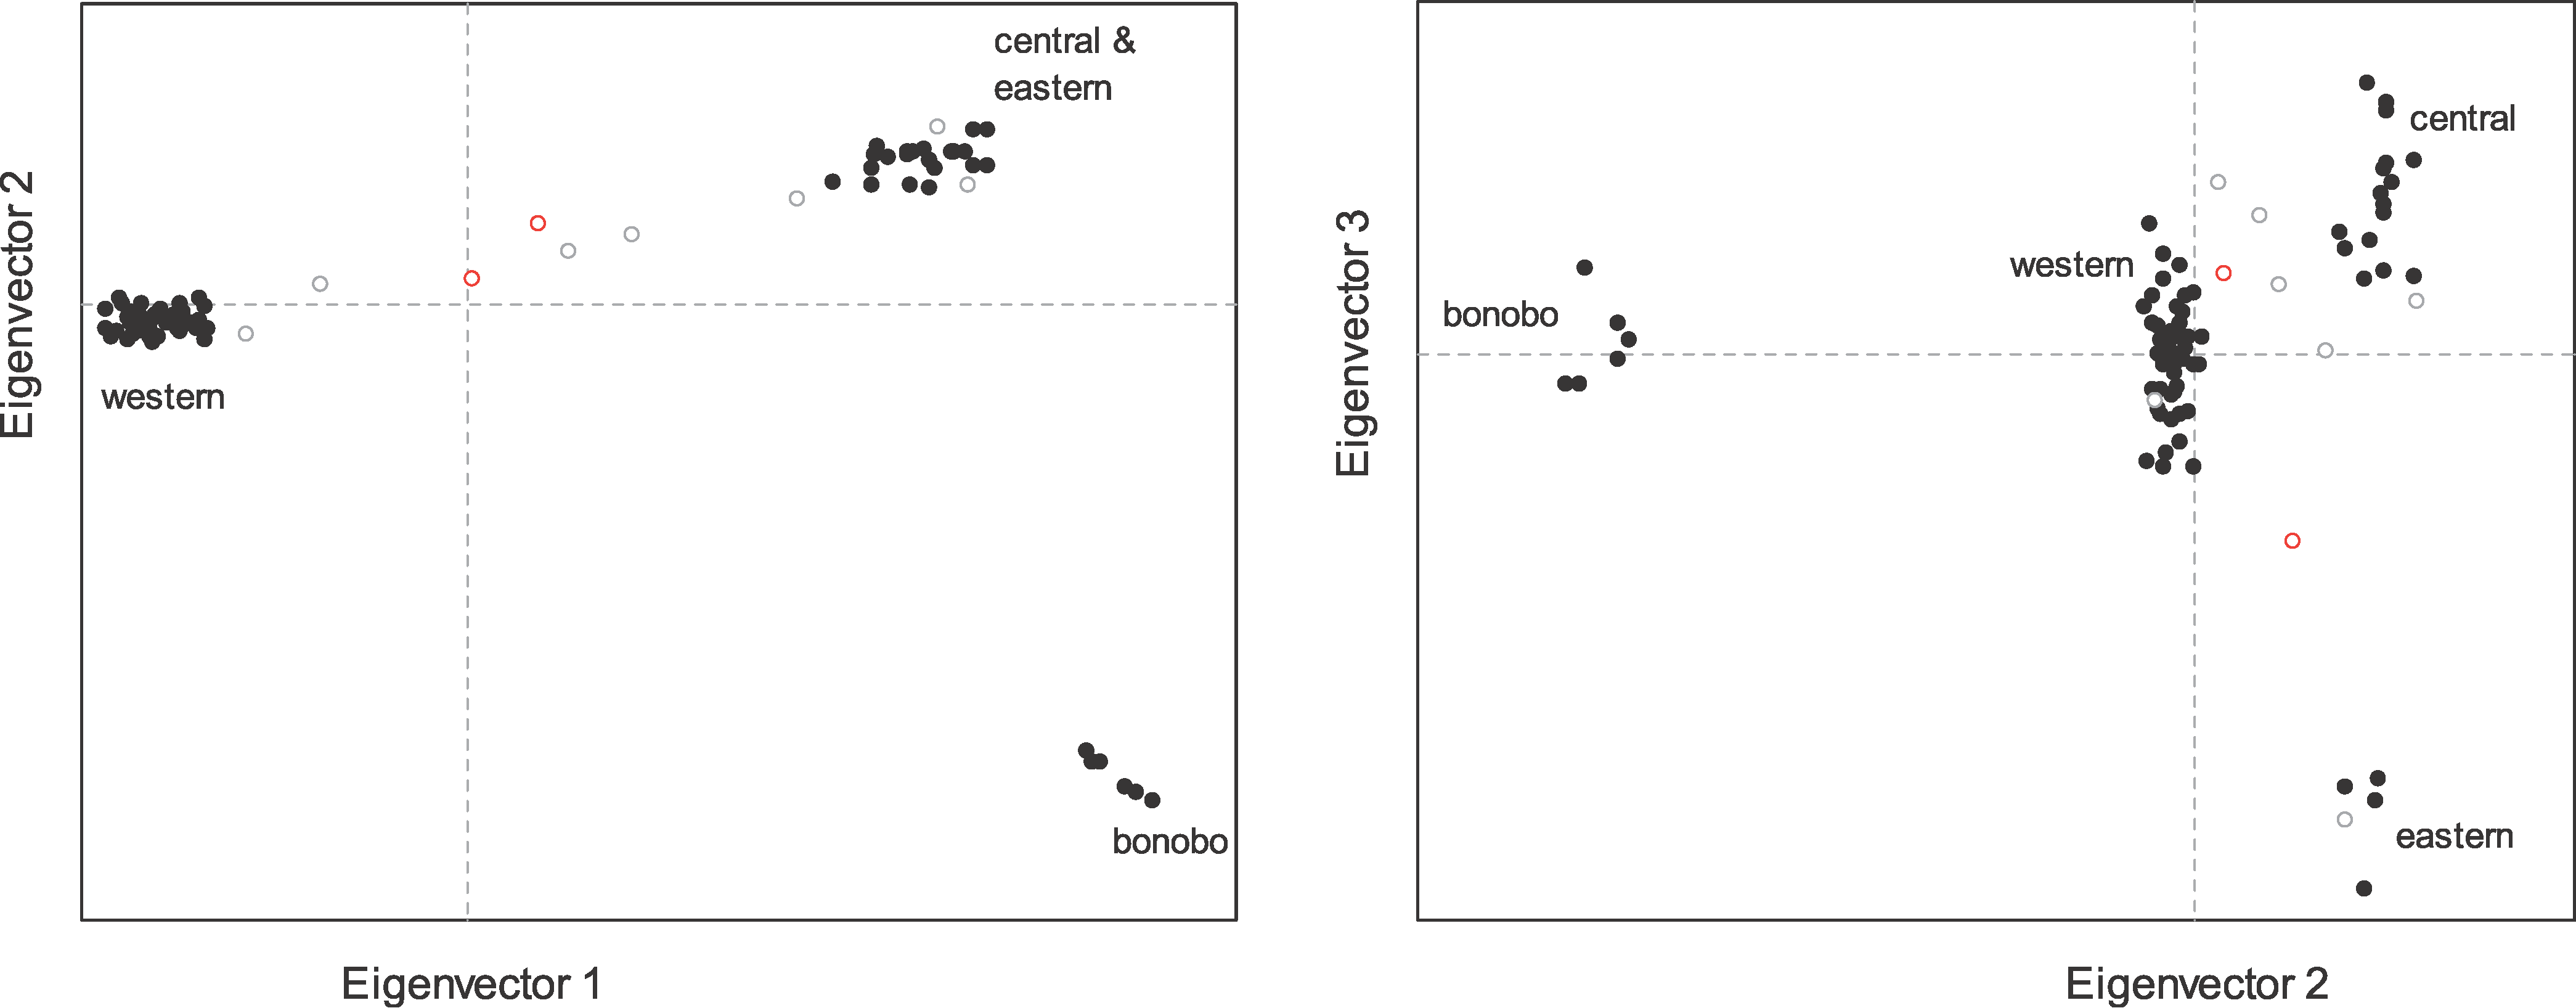
\includegraphics[width=
%   \textwidth]{figures/Becquet_et_al_STRUCTURE_journal_pgen_0030066_g002.png}
%   \caption{ Principal Component Analysis by Becquet {\it et al.} (PLOS Genetics
%     2007) using the same chimpanzee data as in Figure
%     \ref{fig:chimp_structure}. Here they plot the location of each individual
%     on the first two principal components (called eigenvectors) in the left
%     panel, and on the second and third principal components (eigenvectors) in
%     the right panel.  Becquet {\it et al.}'s caption reads: {\it ``PCA, Without
%       Using Population Labels, Divides the 84 Chimpanzees into Four Apparently
%       Discontinuous Populations of Western, Central, Eastern, and Bonobo. Plots
%       of eigenvectors 1 versus 2, and eigenvectors 2 versus 3, show clustering
%       into populations, with the expected assignments for the 75 individuals
%       identified as all of one ancestry by STRUCTURE (solid circles). The nine
%       individuals identified by STRUCTURE as hybrids (open circles) are for the
%       most part identified as hybrids by PCA as well. There are two individuals
%       (red open circles) reported as being of a particular population but that
%       in fact appear to be hybrids: number 23, reported as eastern but in fact
%     a western-eastern hybrid, and number 54, a wild-born individual reported as
%   western but in fact a western-central hybrid.''. } Note that PC1 mostly
%   separates Western chimps from the others, PC2 separates bonobos from all the
% three groups of common chimpanzee. While PC3 separates the Eastern chimp
% samples from the others. Note also how the hybrid individuals (open black and
% red circles) tend to fall intermediate between groups.}

% \label{fig:chimp_PCA}

% % http://journals.plos.org/plosgenetics/article?id=10.1371%2Fjournal.pgen.0030066
% %======= Individuals 76–78 are reported hybrids. Only two individuals with a
% %$>5\%$ proportion of ancestry in more than one inferred cluster are wild born:
% %number 54 and number 17. Red, central; blue, eastern; green, western; yellow,
% %bonobo.''}
% \end{figure}

\newpage
\subsection{Correlations between loci, linkage disequilibrium, and recombination}

%</source-file>

Up to now we have been interested in correlations between alleles at the same
locus, e.g. correlations within individuals (inbreeding) or between individuals
(relatedness). We have seen how relatedness between parents affects the extent
to which their offspring is inbred. We now turn to correlations between alleles
at different loci. To understand correlations between loci we need to
understand recombination.\\


\paragraph{Recombination} 

Let us consider a heterozygous individual, containing $AB$ and $ab$ haplotypes.
If no recombination occurs between our two loci in this individual, then these
two haplotypes will be transmitted intact to the next generation. While if a
recombination (i.e. an odd number of crossing over events) occurs between the
two parental haplotypes, then $\nicefrac{1}{2}$ the time the child receives a
$Ab$ haplotype and $\nicefrac{1}{2}$ the time the child receives a $aB$
haplotype. Effectively, recombination breaks up the association between loci.
We'll define the recombination fraction ($r$) to be the probability of an odd
number of crossing over events between our loci. In practice we'll often be
interested in relatively short regions such that recombination is relatively
rare, and so we might think that $r=r_{BP}L \ll 1$, where $r_{BP}$ is the
average recombination rate per base pair (typically $\sim 10^{-8}$) and L is
the number of base pairs separating our two loci.\\


\paragraph{Linkage disequilibrium}

The (horrible) phrase linkage
disequilibrium (LD) refers to the statistical non-independence
(i.e. a correlation)  of
alleles in a population at different loci. Our two biallelic loci, which segregate alleles $A/a$ and $B/b$, have allele
frequencies of $p_A$ and $p_B$ respectively. The frequency of the two locus haplotype is $p_{AB}$,
and likewise for our other three combinations. If our loci were
statistically independent then $p_{AB} = p_Ap_B$, otherwise $p_{AB} \neq p_Ap_B$
We can define a covariance between the $A$ and $B$ alleles at our two loci as
\begin{equation}
D_{AB} = p_{AB} - p_Ap_B
\end{equation}
and likewise for our other combinations at our two loci
($D_{Ab},~D_{aB},~D_{ab}$).
Gametes with two similar case alleles (e.g. A and B, or a and b) are known as \emph{coupling} gametes, and those with different case alleles are known as repulsion gametes (e.g. a and B, or A and b). Then, we can think of $D$ as measuring the \emph{excess} of coupling to repulsion gametes.
These $D$ statistics are all closely
related to each other as $D_{AB} = - D_{Ab}$ and so on. Thus we only
need to specify one $D_{AB}$ to know them all, so we'll drop the
subscript and just refer to $D$. Also a handy result is that we can rewrite our haplotype
frequency $p_{AB}$ as
\begin{equation}
p_{AB} = p_Ap_B+D. \label{eqn:ABviaD}
\end{equation}
If $D=0$ we'll say the two loci are in linkage equilibrium, while if
$D>0$ or $D<0$ we'll say that the loci are in linkage
disequilibrium (we'll perhaps want to test whether $D$ is
statistically different from $0$ before making this choice). You should be careful to keep the concepts of linkage
and linkage disequilibrium separate in your mind. Genetic linkage refers to the
linkage of multiple loci due to the fact that they
are transmitted through meiosis together (most often because the
loci are on the same chromosome). Linkage disequilibrium merely refers
to the covariance between the alleles at different loci, this may in
part be due to the genetic linkage of these loci but does not
necessarily imply this (e.g. genetically unlinked loci can be in LD
due to population structure). \\

\begin{question} 
You genotype 2 bi-allelic loci (A \& B) segregating in two mouse subspecies (1 \& 2) which mate randomly among themselves, but have not historically interbreed since they speciated. On the basis of previous work you estimate that the two loci are separated by a recombination fraction of 0.1. The frequencies of haplotypes in each population are:
\begin{center}
\begin{tabular}{|c|cccc|}
\hline
Pop    & $p_{AB}$    & $p_{Ab}$ &    $p_{aB}$ &    $p_{ab}$\\
\hline
1 &    .02    & .18 &     .08 &    .72\\
2&    .72 &    .18 &    .08 &    .02\\
\hline
\end{tabular}
\end{center}

{\bf A)} How much LD is there within populations, i.e. estimate D?\\

{\bf B)} If we mixed the two populations together in equal proportions what value would D take before any mating has had the chance to occur? \\
\end{question}



\begin{figure}
\begin{center}
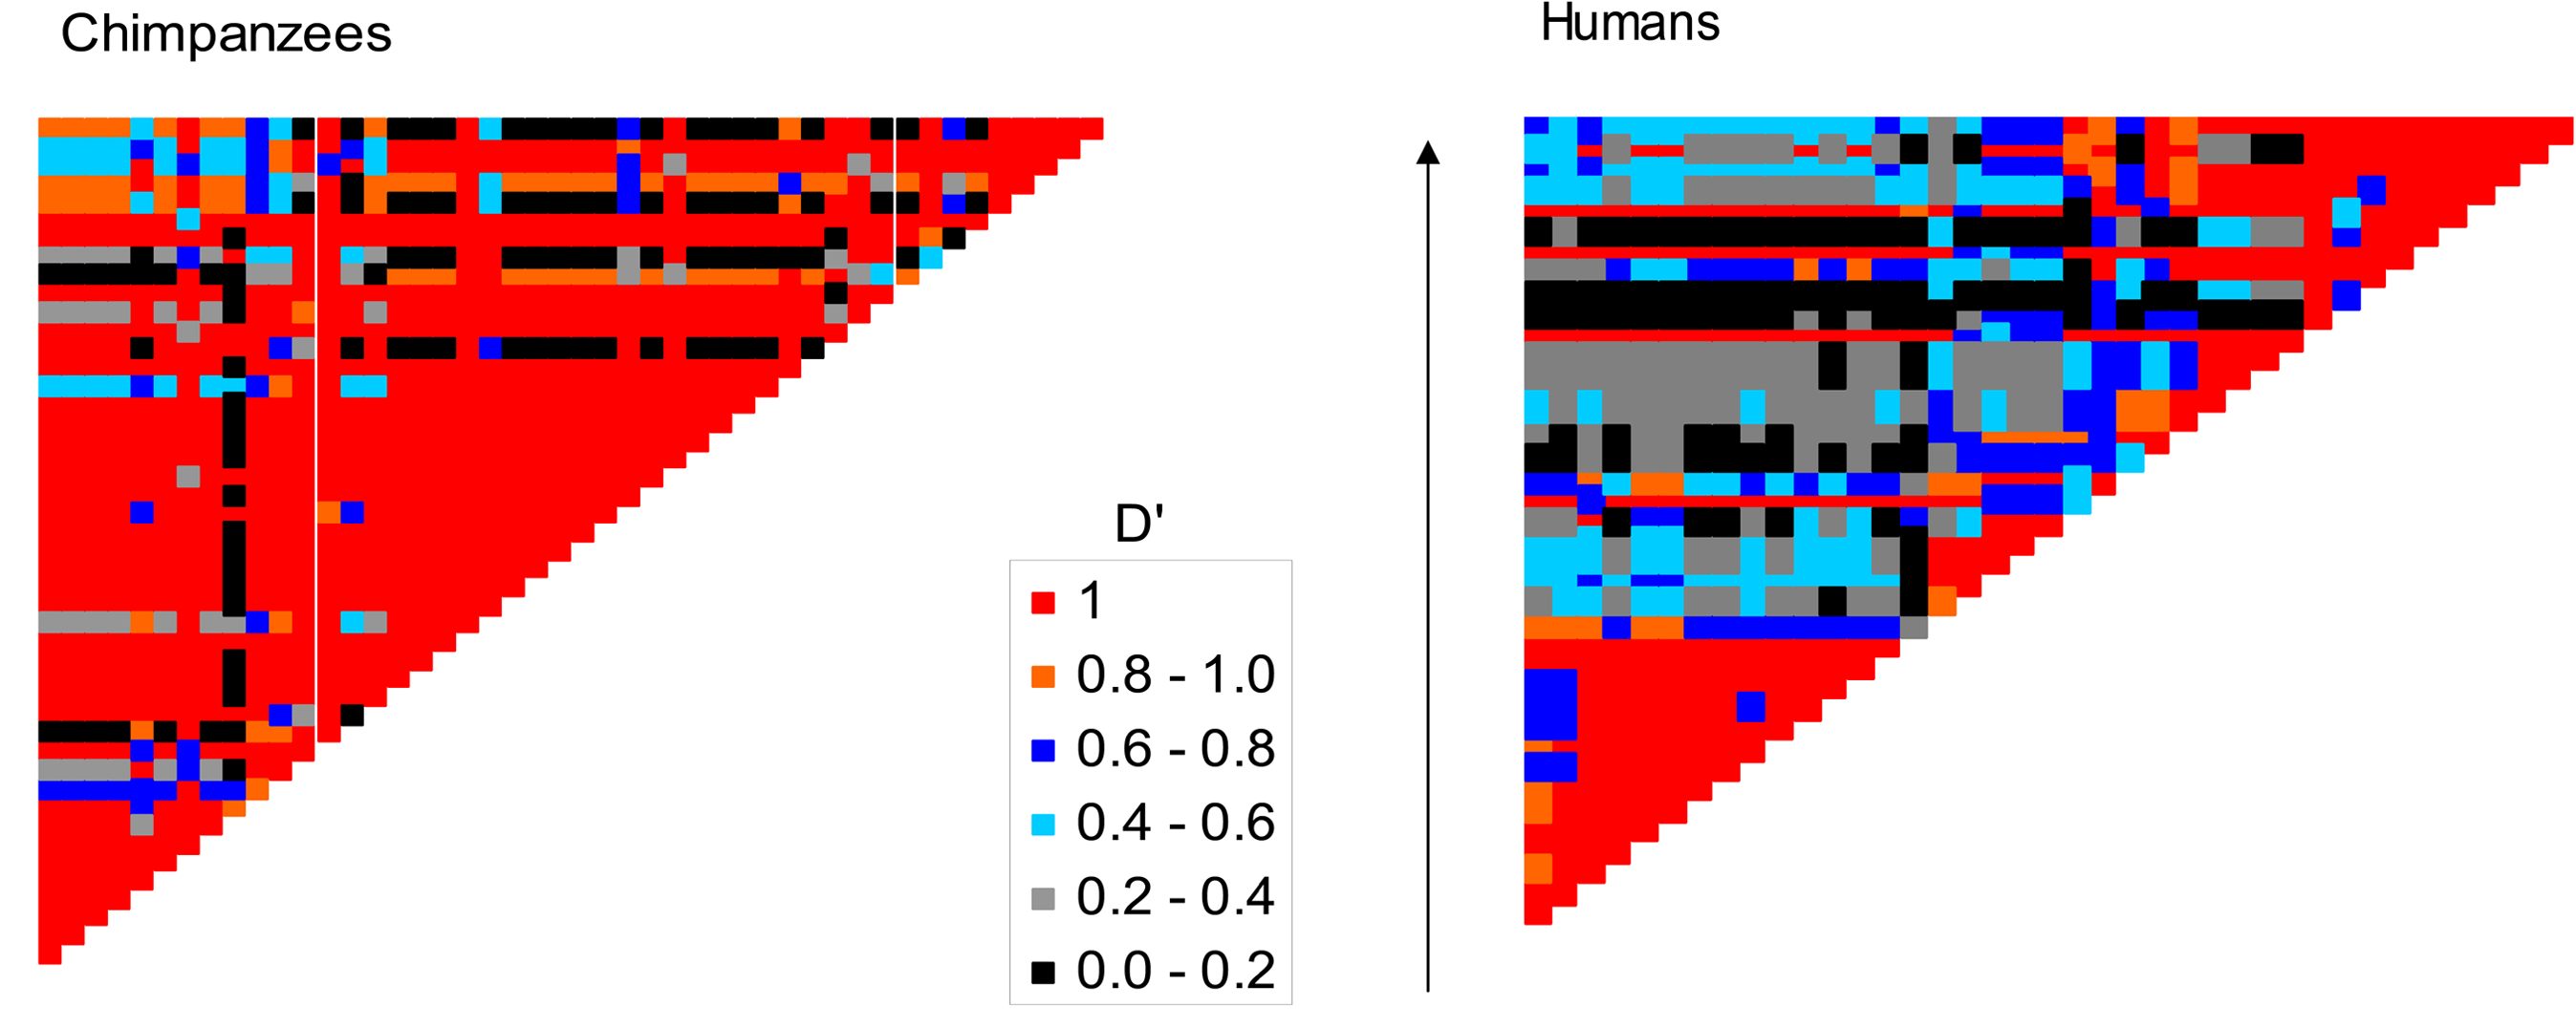
\includegraphics[width= 0.8 \textwidth ]{Journal_figs/alleles_genotypes/TAPS_hotspot/Taps_hotspot.png}
\end{center}
\caption{LD across the TAP2 gene region in a sample of Humans and
  Chimps. The rows and columns are consecutive SNPs, with each cell giving
  the absolute $D^{\prime}$ value between a pair of SNPs. Note that these
are different sets of SNPs in the two species, as shared polymorphisms
are very rare.} \label{fig:TAPS_hotspot}
\end{figure}

Our linkage  disequilibrium statistic $D$ depends strongly on the
allele frequencies of the two loci involved. One common way to
partially remove this dependence, and make it more comparable across
loci, is to divide $D$ through by its the maximum possible value given
the frequency of the loci. This normalized statistic is called
$D^{\prime}$ and vaies between $+1$ and $-1$. In Figure
\ref{fig:TAPS_hotspot} there's an example of LD across the TAP2 region
in human and chimp. Notice how physically close SNPs, i.e. those close
to the diagonal, have higher absolute values of $D^{\prime}$ as
closely linked alleles are separated by recombination less often
allowing high levels of LD to accumulate. Over large physically
distances, away from the diagonal, there is lower $D^{\prime}$. This is
especially notable in humans as there is an intense, human-specific recombination
hotspot in this region, which is breaking down LD between opposite
sides of this region. 

Another common statistic for summarizing LD is $r^2$ which we write as
\begin{equation}
r^2 = \frac{D^2}{p_A(1-p_A) p_B(1-p_B) }
\end{equation}
as $D$ is a covariance, and $p_A(1-p_A) $ is the variance of an allele
drawn at random from locus $A$, $r^2$ is the squared correlation
coefficient.  Note that this $r$ in $r^2$ is NOT the recombination
fraction.   \\

\begin{marginfigure}
\begin{center}
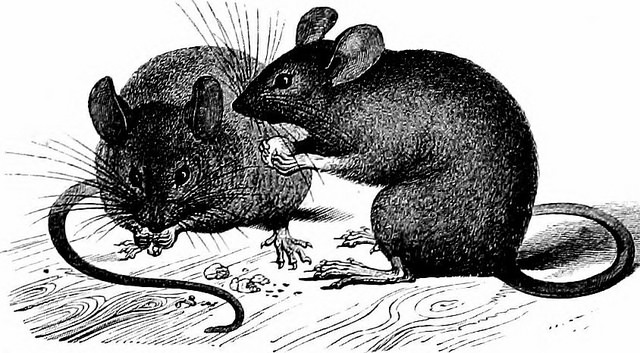
\includegraphics[width=\textwidth]{illustration_images/alleles_genotypes/Mus_musculus/20746324002_e014b4fcc6_z.jpg}
\end{center}
\caption{{\it Mus musculus}. A history of British quadrupeds, including the Cetacea. 1874. Bell T., Tomes, R. F.m Alston E. R.} \label{fig:Mouse}
\end{marginfigure}



Figure \ref{fig:Mouse_LD} shows $r^2$ pairs of SNPs at
various physical distances in two population samples of {\it Mus musculus
  domesticus}. Again LD is highest between physically close markers as LD is being generated faster than it can be
decayed via recombination; more distance marker have much lower LD as
here recombination is winning out. Note how the decay of LD is much
slower in the advanced-generation cross population, where LD persists
across megabases. due to the limited number of generations for recombination
since the cross was created.


\begin{figure}
\begin{center}
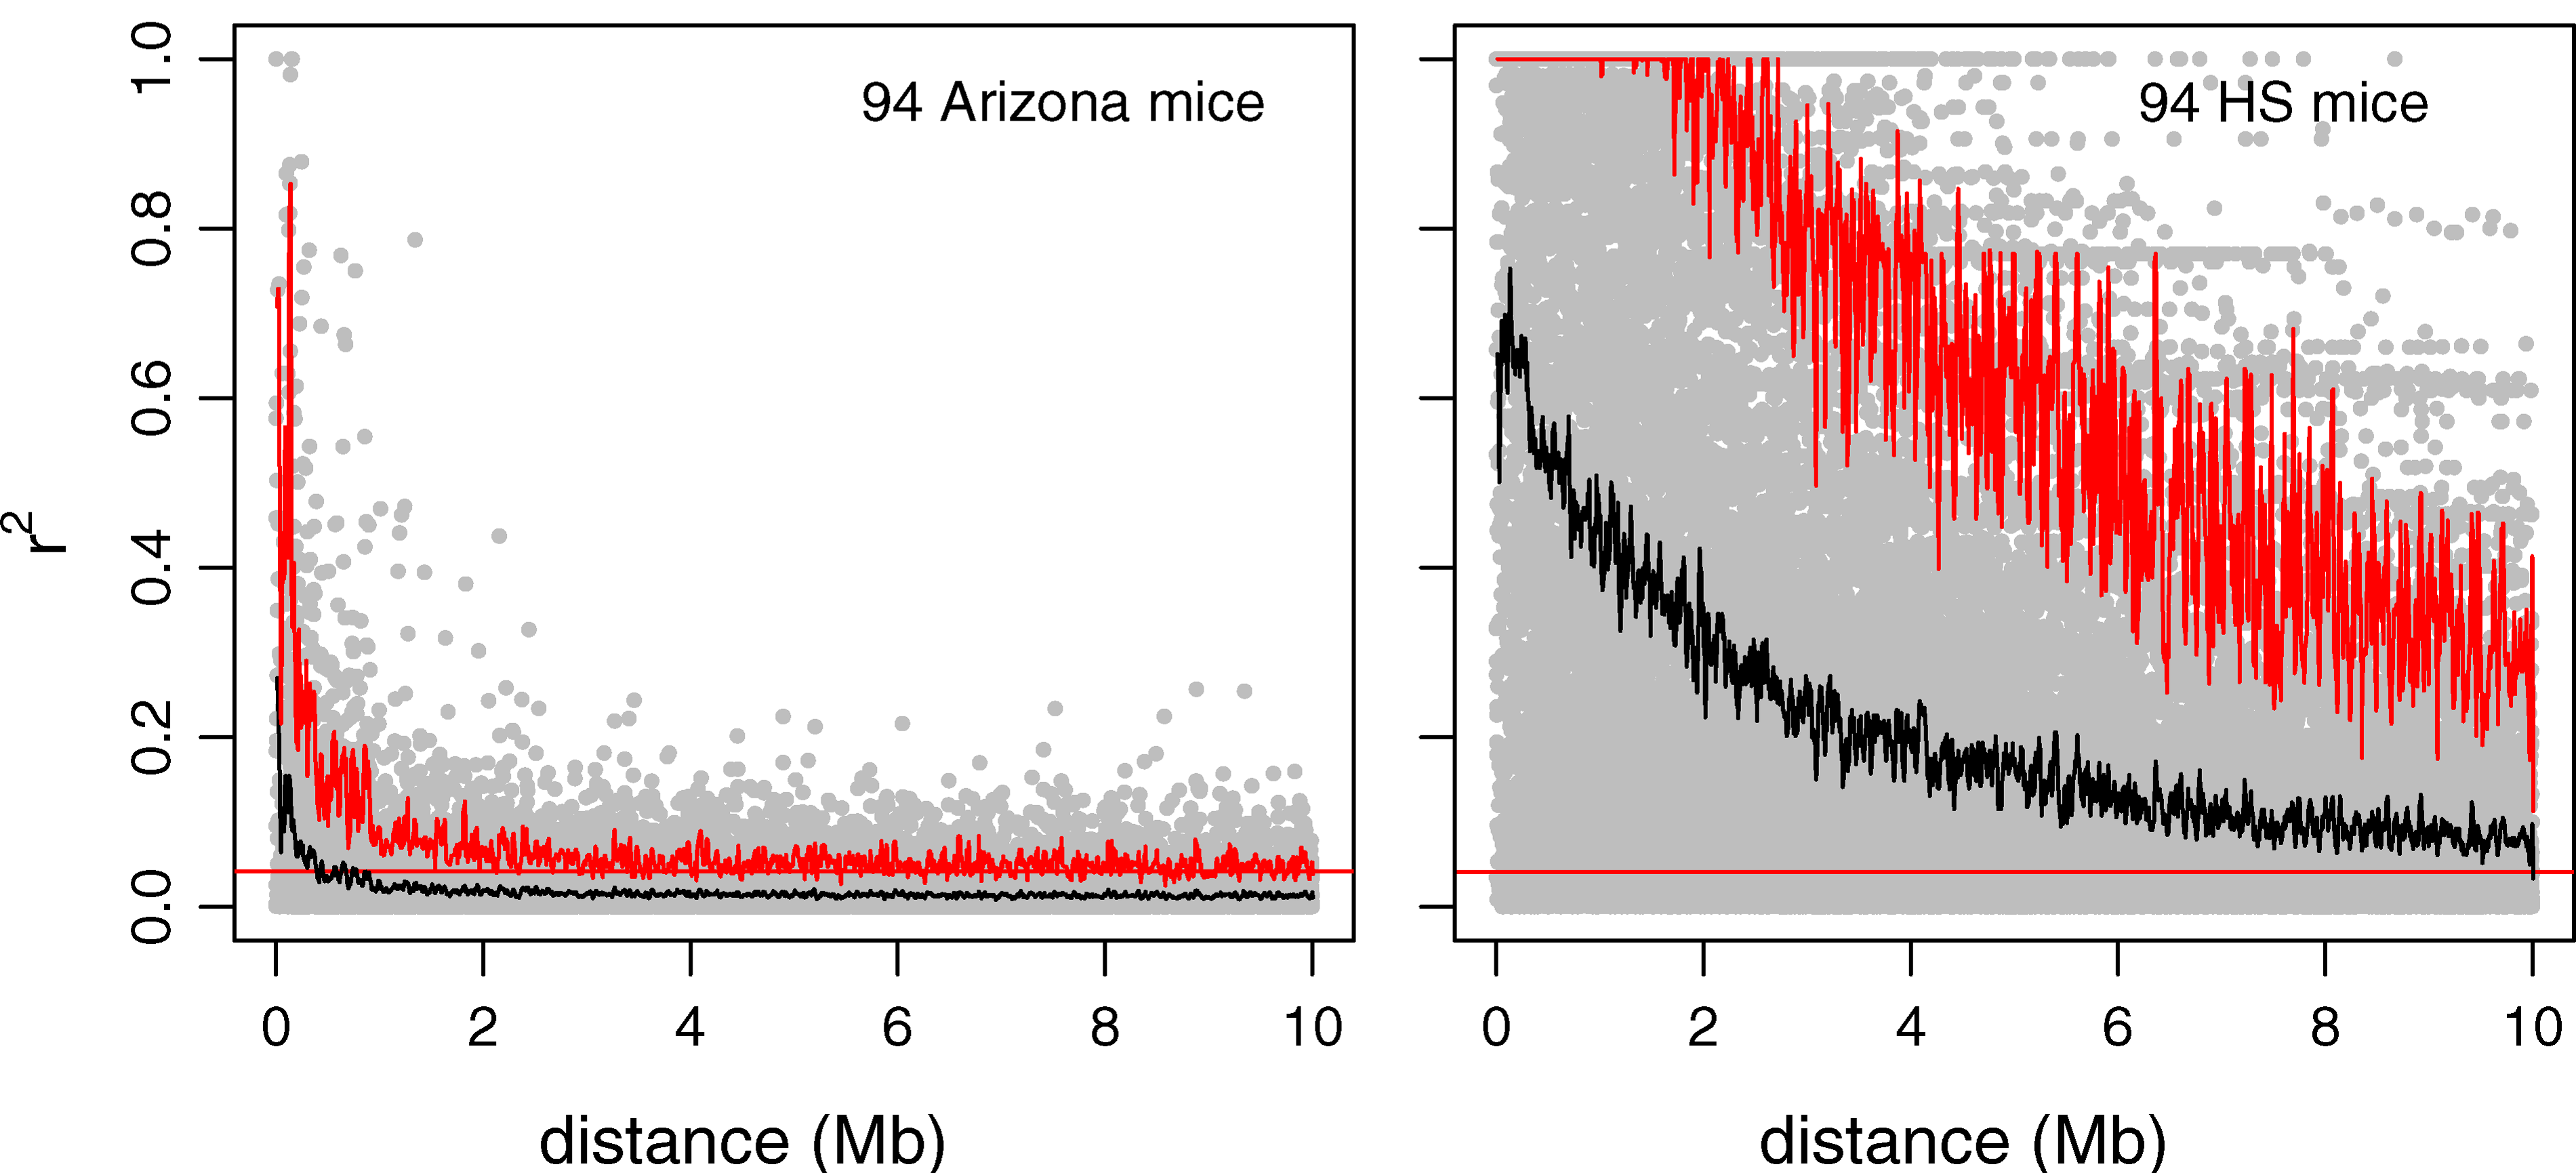
\includegraphics[width=0.8 \textwidth]{Journal_figs/alleles_genotypes/mouse_LD/mouse_LD_Laurie_et_al.png}
\end{center}
\caption{The decay of LD for autosomal SNP in {\it Mus musculus
  domesticus}, as measured by $r^2$, in a wild-caught mouse population
  from Arizona and a set of advanced-generation crosses between inbred lines of lab mice. Each dot gives the $r^2$ for a
  pair of SNPs a given physical distance apart, for a total of $\sim
  3000$ SNPs. The solid black line gives the mean, the jagged the
  $95^{th}$ percentile, and the flat red line a cutoff for
  significant $LD$. From \citeauthor{Laurie:07}. } \label{fig:Mouse_LD}
\end{figure}


\paragraph{The generation of LD.}
Various population genetic forces can generate LD. Selection can generate LD by favouring particular combinations of
alleles. Genetic drift will also generate LD, not because particular
combinations of alleles are favoured, but simply because at random particular
haplotypes can by chance drift up in frequency. Mixing between
divergent populations can also generate LD, as we saw in mouse
Question above. 




\paragraph{The decay of LD due to recombination}

We will now examine what happens to LD over the generations if we
only allow recombination to occur in a very large population (i.e. no
genetic drift, i.e. the frequencies of our loci follow their expectations). To do so consider the frequency of our $AB$ haplotype in the next generation
$p_{AB}^{\prime}$. We lose a fraction $r$ of our $AB$ haplotypes to
recombination ripping our alleles apart but gain a fraction $rp_A p_B$ per generation from other
haplotypes recombining together to form $AB$ haplotypes. Thus in the
next generation
\begin{equation}
p_{AB}^{\prime} = (1-r)p_{AB} + rp_Ap_B
\end{equation}
this last term here is $r(p_{AB}+p_{Ab})(p_{AB}+p_{aB})$, which
multiplying this out is the
probability of recombination in the different diploid genotypes that
could generate a $p_{AB}$ haplotype. \\

We can then write the change in the frequency of the $p_{AB}$
haplotype as
\begin{equation}
\Delta p_{AB} = p_{AB}^{\prime} -p_{AB} = -r p_{AB} + rp_Ap_B = - r D
\end{equation}
so recombination will cause a decrease in the frequency of $p_{AB}$ if
there is an excess of $AB$ haplotypes within the population ($D>0$), and an
increase if there is a deficit of $AB$ haplotypes within the
population ($D<0$). Our LD in the next generation is $D^{\prime} =
p_{AB}^{\prime}$, so we can rewrite the above eqn. in terms of the
$D^{\prime} $
\begin{equation}
D^{\prime}= (1-r) D
\end{equation}
so if the level of LD in generation $0$ is $D_0$ the level $t$
generations later ($D_t$) is
\begin{equation}
D_t=  (1-r)^t D_0
\end{equation}
so recombination is acting to decrease LD, and it does so
geometrically at a rate given by $(1-r)$. If $r \ll 1$ then we can
approximate this by an exponential and say that   
\begin{equation}
D_t \approx  D_0 e^{-rt}  \label{eqn_LD_decay}
\end{equation}\\



%{\bf Q}\arabic{Question} \refstepcounter{Question}  
\begin{question} 
You find a hybrid population between the two mouse subspecies
described in the question above, which appears to be comprised of equal proportions of ancestry from the two subspecies.  You estimate LD between the two markers to be 0.0723. Assuming that this hybrid population is large and was formed by a single mixture event, can you estimate how long ago this population formed? \\
\end{question}

%
\begin{marginfigure}
\begin{center}
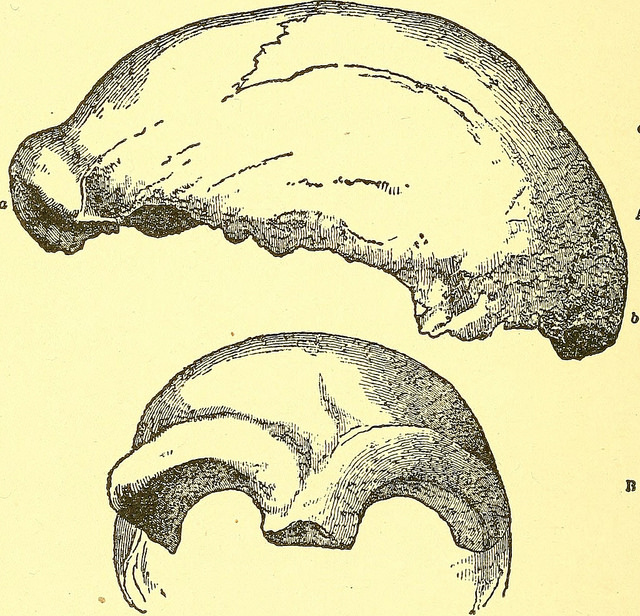
\includegraphics[width=\textwidth]{illustration_images/alleles_genotypes/Neanderthal/14800262343_f21929987a_z.jpg}
\end{center}
\caption{The earliest discovered fossil of a Neanderthal, fragments of
  a skull found in a cave in the Neander Valley in Germany. Man's place in nature. 1890. Huxley, T. H.} \label{fig:Mouse_LD}
\end{marginfigure} 

A particularly striking example of the decay of LD generated by
the mixing of populations is offered by the LD created by the
interbreeding on humans and Neanderthals. Neanderthals and modern
Humans diverged from each other likely over half a million years ago,
allowing time for allele frequency differences to accumulate between
the species. The two population spread back into secondary contact, when
humans moved out of Africa over the past hundred thousand years or
so. One of the most exciting findings from the sequencing of the
Neanderthal genome was that modern-day people with Eurasian ancestry
carry a few percent of their genome derived from the Neanderthal
genome, via interbreeding during this secondary contact. To date the timing of this
interbreeding \citeauthor{Sankararaman:12} looked at the LD in modern
humans between pairs of alleles found to be derived the Neanderthal
genome (and nearly absent from African populations). 
In Figure \ref{fig:LD_Neanderthal} we show the average LD between these loci
is shown as a function of the genetic distance ($r$) between them from
the works of 
\citeauthor{Sankararaman:12}.
\begin{figure}
\begin{center}
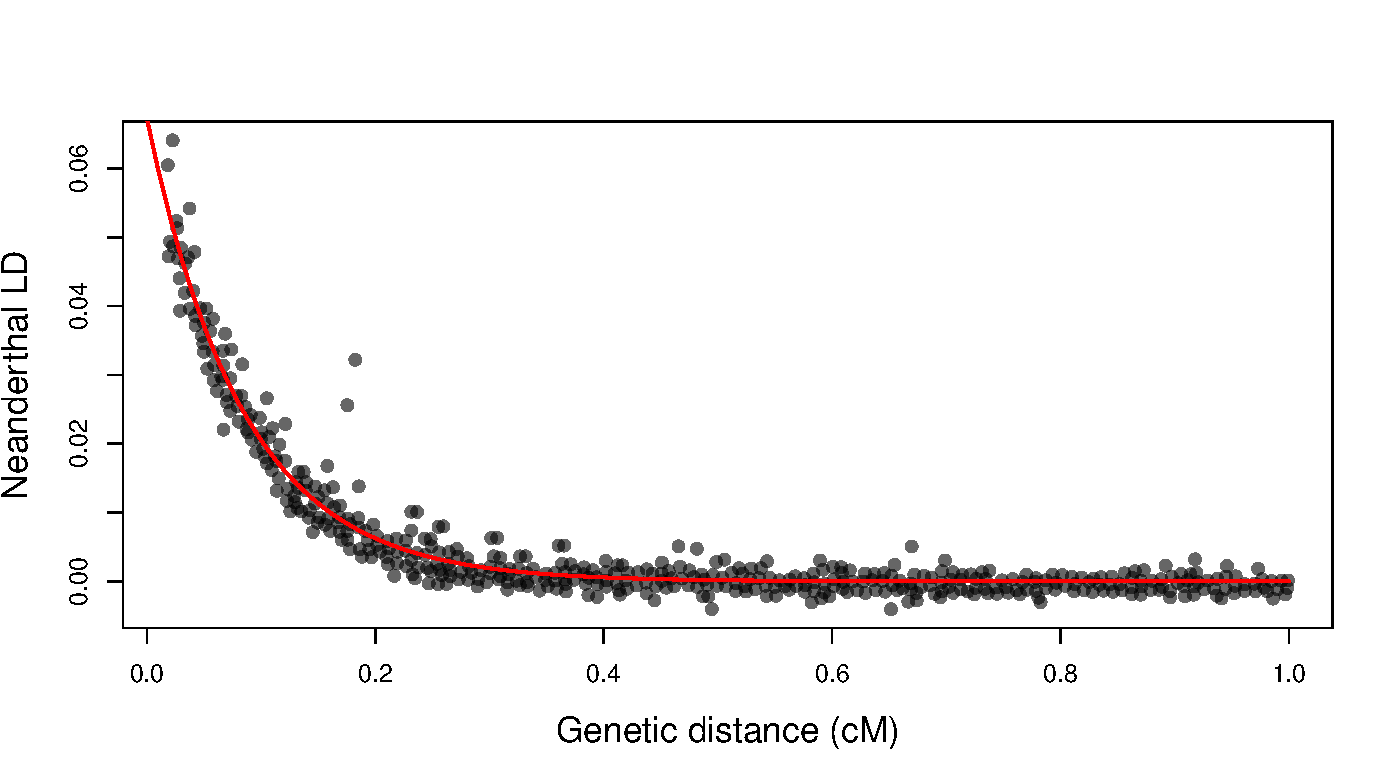
\includegraphics[width=0.8 \textwidth]{Journal_figs/alleles_genotypes/Neanderthal_LD/European_neanderthal_LD.pdf}
\end{center}
\caption{ } \label{fig:LD_Neanderthal}
\end{figure}

We can fit the exponential decay of LD with $r$ predicted by eqn \eqref{eqn_LD_decay} to the data points in this figure,
the fit is shown as a red line. Doing this we estimate $t=1200$
generations, or about 35 thousand years (using a human generation time of 29
years). Thus the LD, in modern Eurasians, between alleles derived from
the interbreeding Neanderthal represents over thirty thousand years of
recombination slowly breaking down these old
associations. \marginnote{The calculation done by
  \citeauthor{Sankararaman:12} is actually a bit more involved as they
account for inhomogenity in recombination rates and arrive at a date
of  47,334–63,146 years.}






%\subsection{Testing for departures from HWE.}
%Note the form of $\hat{F}$ \eqref{eqn:FhatHO} is the same as the $X^2$
%statistic, and so we can test for a deviation from hardy-weinberg  $X^2$


%\subsection{Population structure}
%The question naturally arises at this point: what reference population
%(i.e. what allele frequency) do we use to calculate $\hat{F}$? If we are %calculating the inbreeding coefficient
%of an English person do we use the frequencies of the town of that
%person, of England, of the United Kingdom, or of the World?



%\gc{Include the HapMap exercise here?}


%==One locus models of selection==
%<source-file filename="one_loc_sel_models.tex" display="one_loc_sel_models.wrapped.latexml.xhtml">


